\documentclass{article}

% if you need to pass options to natbib, use, e.g.:
%     \PassOptionsToPackage{numbers, compress}{natbib}
% before loading neurips_2025

% The authors should use one of these tracks.
% Before accepting by the NeurIPS conference, select one of the options below.
% 0. "default" for submission
 \usepackage{neurips_2025}
 \usepackage{graphicx}
% the "default" option is equal to the "main" option, which is used for the Main Track with double-blind reviewing.
% 1. "main" option is used for the Main Track
%  \usepackage[main]{neurips_2025}
% 2. "position" option is used for the Position Paper Track
%  \usepackage[position]{neurips_2025}
% 3. "dandb" option is used for the Datasets & Benchmarks Track
 % \usepackage[dandb]{neurips_2025}
% 4. "creativeai" option is used for the Creative AI Track
%  \usepackage[creativeai]{neurips_2025}
% 5. "sglblindworkshop" option is used for the Workshop with single-blind reviewing
 % \usepackage[sglblindworkshop]{neurips_2025}
% 6. "dblblindworkshop" option is used for the Workshop with double-blind reviewing
%  \usepackage[dblblindworkshop]{neurips_2025}

% After being accepted, the authors should add "final" behind the track to compile a camera-ready version.
% 1. Main Track
 % \usepackage[main, final]{neurips_2025}
% 2. Position Paper Track
%  \usepackage[position, final]{neurips_2025}
% 3. Datasets & Benchmarks Track
 % \usepackage[dandb, final]{neurips_2025}
% 4. Creative AI Track
%  \usepackage[creativeai, final]{neurips_2025}
% 5. Workshop with single-blind reviewing
%  \usepackage[sglblindworkshop, final]{neurips_2025}
% 6. Workshop with double-blind reviewing
%  \usepackage[dblblindworkshop, final]{neurips_2025}
% Note. For the workshop paper template, both \title{} and \workshoptitle{} are required, with the former indicating the paper title shown in the title and the latter indicating the workshop title displayed in the footnote.
% For workshops (5., 6.), the authors should add the name of the workshop, "\workshoptitle" command is used to set the workshop title.
% \workshoptitle{WORKSHOP TITLE}

% "preprint" option is used for arXiv or other preprint submissions
 % \usepackage[preprint]{neurips_2025}

% to avoid loading the natbib package, add option nonatbib:
%    \usepackage[nonatbib]{neurips_2025}

\usepackage[utf8]{inputenc} % allow utf-8 input
\usepackage[T1]{fontenc}    % use 8-bit T1 fonts
\usepackage{hyperref}       % hyperlinks
\usepackage{url}            % simple URL typesetting
\usepackage{booktabs}       % professional-quality tables
\usepackage{amsfonts}       % blackboard math symbols
\usepackage{nicefrac}       % compact symbols for 1/2, etc.
\usepackage{microtype}      % microtypography
\usepackage{xcolor}         % colors
\usepackage{amsmath}
\usepackage{amssymb}        % for additional math symbols like \blacksquare
\usepackage{float}          % for fixed figure placement with [H]
\usepackage{algorithm}      % for algorithms
\usepackage{algpseudocode}  % for algorithm pseudocode

% Note. For the workshop paper template, both \title{} and \workshoptitle{} are required, with the former indicating the paper title shown in the title and the latter indicating the workshop title displayed in the footnote. 
\title{Scaling Flow Matching Models at Inference-Time by Search and Path Exploration}

\begin{document}


\maketitle


\begin{abstract}
Inference‑time compute scaling has become a powerful means of improving discrete generative models, yet its counterpart for continuous‑time generative models remains under‑explored. We close this gap for flow‑matching (FM) models, whose deterministic ordinary‑differential (ODE) and stochastic differential (SDE) samplers underpin state‑of‑the‑art continuous generative models in domains such as image‑generation and protein‑folding. We introduce an inference‑time strategy that injects analytically constructed divergence‑free perturbations into the learned velocity field during ODE sampling. The perturbations preserve the method's defining linear interpolation path and exactly maintain the continuity equation, ensuring that probability mass is conserved while enabling the sampler to explore high quality trajectories, without modifying trained parameters. We additionally include SDE sampling as an alternative approach. Experiments on ImageNet and FoldFlow demonstrate our methods ability to trade-off computation time with sampling quality over multiple key metrics for each domain. Our work positions inference‑time scaling as a principled, training‑free lever for enhancing flow‑matching models and invites future exploration across diverse continuous generative tasks.
\end{abstract}


\section{Introduction}

Inference-time compute scaling has emerged as a transformative paradigm in generative modeling, enabling performance improvements through increased computational resources at test time without requiring model retraining. While this approach has shown remarkable success in discrete domains—from language models like OpenAI's O1~\cite{openai2024o1} to diffusion models for image generation~\cite{ma2025diffits}—its application to continuous-time generative models remains largely unexplored.

Flow Matching (FM)~\cite{lipman2023fm} has established itself as a leading framework for continuous generative modeling, offering deterministic sampling through ordinary differential equations (ODEs) and achieving state-of-the-art results across diverse domains including image generation~\cite{esser2024scaling} and protein design~\cite{wu2024foldflow}. However, the deterministic nature of FM sampling presents a fundamental challenge for inference-time scaling: unlike diffusion models that naturally provide stochasticity through noise injection, FM models follow a single, predetermined trajectory from noise to data, leaving limited opportunities for exploring alternative generation paths.

This work introduces the first principled approach to inference-time scaling for flow matching models. Our key insight is that we can inject carefully constructed divergence-free perturbations into the learned velocity field during sampling, creating a family of alternative ODE trajectories while preserving the fundamental mathematical properties of the original model. Specifically, our perturbations maintain the continuity equation at the trajectory level, ensuring exact conservation of probability mass throughout the generation process.

We make several key contributions:

\textbf{Theoretical Framework:} We prove that adding divergence-free perturbations to the velocity field preserves the continuity equation, providing mathematical guarantees that our modifications do not violate the underlying probability flow. Our approach maintains the linear interpolation paths and ODE structure that define flow matching, unlike concurrent work that converts to SDE sampling.

\textbf{Practical Algorithms:} We develop two complementary strategies: (1) divergence-free path exploration that generates multiple trajectories from a single initial condition, and (2) a two-stage approach combining random search over initial conditions with divergence-free exploration around promising candidates. This mirrors the exploration-exploitation tradeoff in reinforcement learning.

\textbf{Empirical Validation:} We demonstrate the effectiveness of our approach across two distinct domains. On ImageNet 256×256 using SiT-XL/2, our methods achieve significant improvements in FID, Inception Score, and DINO accuracy as compute budget increases. On protein design using FoldFlow, we show substantial improvements in structural quality (TM-score) from 0.743 to 0.868, establishing the cross-domain applicability of our approach.

\textbf{Methodological Insights:} Our experiments reveal that different inference-time scaling strategies excel under different conditions: random search provides broad exploration particularly effective for discrete sequence-structure relationships, while divergence-free perturbations enable focused local search around high-quality regions. The combination of both approaches consistently outperforms either method in isolation.

Our work establishes inference-time scaling as a viable and principled approach for enhancing flow matching models, opening new directions for improving continuous generative models across scientific and creative applications without the computational cost of retraining.


\section{Preliminaries}
\label{sec:preliminaries}

\subsection{Flow Matching}

Flow Matching (FM)~\cite{lipman2023fm} defines a continuous bridge between a reference distribution \(\pi_{\mathrm{ref}}\), typically a standard Gaussian, and a data distribution \(\pi_{\mathrm{data}}\), by modeling trajectories \(x_t\) that interpolate linearly between samples \(x_0 \sim \pi_{\mathrm{ref}}\) and \(x_1 \sim \pi_{\mathrm{data}}\). This is done via a learned velocity field \(v_\theta(x, t)\) that satisfies the probability-flow ODE:
\[
\frac{dx_t}{dt} = v_\theta(x_t, t), \quad x_t = (1 - t)x_0 + t x_1, \quad t \in [0,1].
\]
To train \(v_\theta\), a supervised loss is used where the ground truth velocity is known analytically:
\[
v^\star(x_t, t) = x_1 - x_0.
\]
This target arises because \(\frac{dx_t}{dt} = x_1 - x_0\) under linear interpolation. The training loss is then
\[
\mathcal{L}_{\mathrm{FM}} = \mathbb{E}_{x_0 \sim \pi_{\mathrm{ref}}, x_1 \sim \pi_{\mathrm{data}}, t \sim \mathcal{U}[0,1]} \left[ \left\| v_\theta(x_t, t) - (x_1 - x_0) \right\|^2 \right].
\]
Unlike diffusion models that rely on stochastic sampling from SDEs or discrete Markov chains, FM offers a deterministic, fast, and interpretable sampling process. Because the interpolant is linear and the learned dynamics are smooth, FM enables fewer sampling steps while maintaining sample quality.

\subsection{Minibatch Optimal Transport Flow Matching (OT-FM)}

While FM defines its objective using i.i.d. sample pairs \((x_0, x_1)\), such pairs are typically poorly coupled in high-dimensional space. Minibatch OT-FM~\cite{tong2024otfm} addresses this by using an optimal transport (OT) plan computed within each minibatch to generate more meaningful pairs. That is, given batches \(\{x_{0,i}\}_{i=1}^B\) from \(\pi_{\mathrm{ref}}\) and \(\{x_{1,j}\}_{j=1}^B\) from \(\pi_{\mathrm{data}}\), an optimal permutation matrix \(\pi^\star \in \Pi_B\) is computed to minimize a transport cost:
\[
\pi^\star = \arg\min_{\pi \in \Pi_B} \sum_{i,j} \pi_{ij} \cdot c(x_{0,i}, x_{1,j}),
\]
where \(c(\cdot, \cdot)\) is typically Euclidean distance. This plan yields better-aligned pairs that shorten transport paths, stabilize training, and improve generalization.

\subsection{Stochastic Interpolants: A Unifying Framework}

The stochastic interpolants framework~\cite{ma2024sit} shows that both FM and diffusion models can be described using the same general family of interpolations. A stochastic interpolant is defined by
\[
x_t = a(t) x_0 + b(t) x_1 + \sigma(t) \epsilon, \quad \epsilon \sim \mathcal{N}(0, I),
\]
where \(a(t), b(t)\), and \(\sigma(t)\) are schedule functions satisfying boundary conditions: \(a(0) = 1\), \(b(1) = 1\), \(a(1) = b(0) = 0\), and \(\sigma(0) = \sigma(1) = 0\). This framework can express linear FM, denoising diffusion models, and their hybrids.

Crucially, this allows inference-time reinterpretation of trained models by simply modifying the interpolant schedule. For example, a model trained using FM with linear schedules \((a(t), b(t)) = (1 - t, t)\) and \(\sigma(t) = 0\) can be reinterpreted at test time as a VP diffusion model by using \((a(t), b(t)) = (\cos(\alpha t), \sin(\alpha t))\) and \(\sigma(t) \neq 0\). This reveals a continuum of models and motivates inference-time strategies that leverage the same learned model parameters.

\subsection{Inference-Time Compute Scaling in Generative AI}

Inference-time scaling refers to performance improvements achieved by increasing computational resources \emph{after training}, without modifying model parameters. While generative models have traditionally scaled performance by increasing data, model size, or training compute, recent research has explored whether additional computation at inference can yield better outputs.

In discrete domains such as language modeling, inference scaling has been explored through methods that allocate more compute per query. These include using longer reasoning chains, recursive planning, or verifier-guided editing~\cite{gandhi2024sos, cobbe2021verifiers, lightman2023verify, brown2024llmmonkeys}. Notably, OpenAI's O1 and O3 models~\cite{openai2024o1} and DeepSeek R1~\cite{deepseek2024r1} do not use branching across multiple sampled responses. Instead, they increase inference-time compute by allowing more function evaluations per output, for example via deeper chains-of-thought or tree-based planning structures.

In contrast, recent work in diffusion models has implemented inference-time scaling via **search over generation trajectories**~\cite{ma2025diffits}. Diffusion models naturally provide stochasticity through their noise-injection process. The inference-time scaling diffusion framework identifies that \emph{some initial noises are better than others}, and proposes to search over this noise space using verifiers to guide sample selection. This turns the generation problem into a two-axis search: one axis governs the verifier that provides feedback (e.g., Inception Score, CLIP, DINO), and the other defines the search algorithm (e.g., random search, zero-order optimization, path-space exploration). This approach allows performance to continue improving beyond what is achievable by simply increasing denoising steps.

These developments motivate the need for inference-time scaling in **continuous-time models** such as Flow Matching (FM), which lack natural sources of stochasticity or branching. The key challenge is that FM models sample deterministically via a single integration of the learned velocity field along a fixed interpolant. Our method addresses this by introducing divergence-free perturbations to the velocity field, thereby defining a family of ODEs that maintain the continuity equation but diverge in geometry. This enables principled sampling diversity and verifier-guided branching in FM, filling a crucial gap in inference-time scaling for continuous-time generative models.


\section{Related Work}
\label{sec:related}

\subsection{Inference-Time Scaling for Flow Matching Models}

A concurrent line of work proposes inference-time scaling for flow models by introducing stochasticity and path diversity into the otherwise deterministic sampling process~\cite{kim2025flowits}. This is achieved through a two-step transformation of the learned model: (1) converting the velocity field from the probability flow ODE to a score-based SDE sampler, and (2) replacing the standard linear interpolant with a variance-preserving (VP) interpolant path to enhance exploration.

Specifically, the learned velocity \( u_t(x) \) is used to define the drift term of a reverse-time SDE:
\[
d x_t = f_t(x_t)\,dt + g_t\,dW_t, \quad \text{where } f_t(x_t) = u_t(x_t) - \frac{g_t^2}{2} \nabla \log p_t(x_t).
\]
The score function \( \nabla \log p_t(x_t) \) is estimated analytically from \( u_t \) using the stochastic interpolants framework~\cite{ma2024sit}:
\[
\nabla \log p_t(x_t) = \frac{1}{\sigma_t} \cdot \frac{\alpha_t u_t(x_t) - \dot{\alpha}_t x_t}{\dot{\alpha}_t \sigma_t - \alpha_t \dot{\sigma}_t}.
\]
In parallel, the interpolation path is converted from a linear interpolant \( x_t = (1 - t)x_0 + t x_1 \) to a VP interpolant, such as \( x_t = \alpha_t x_0 + \sigma_t x_1 \) where \(\alpha_t^2 + \sigma_t^2 = 1\). This conversion requires transforming the original velocity field into one compatible with the new interpolant~\cite{kim2025flowits}:
\[
\bar{u}_s(\bar{x}_s) = \frac{\dot{c}_s}{c_s} \bar{x}_s + c_s \dot{t}_s u_{t_s}(\bar{x}_s / c_s),
\]
where \(c_s = \bar{\sigma}_s / \sigma_{t_s}\) and \(t_s = \rho^{-1}(\bar{\rho}(s))\) is defined via signal-to-noise ratio schedules \(\rho(t) = \alpha_t/\sigma_t\), \(\bar{\rho}(s) = \bar{\alpha}_s/\bar{\sigma}_s\).

This approach enables the use of particle sampling strategies originally developed for diffusion models, which benefit from diverse sample paths and stochastic exploration. However, by transforming both the dynamics and the interpolant, the method loses the key benefits of flow matching: fast sampling via few deterministic steps and linear interpolants.

While this work is concurrent to our own, we still differentiate ourselves as our method preserves the original FM structure. We maintain the ODE form of the sampler and the linear interpolant, and introduce diversity solely by injecting divergence-free velocity perturbations during sampling. This guarantees that probability mass is conserved through the continuity equation, while allowing geometrically distinct trajectories for verifier-guided search.

\subsection{Noise Injection while Preserving the Continuity Equation}

A distinct thread of work aims to inject stochasticity during inference without violating the underlying continuity equation that defines the model's evolution. This objective is shared by our divergence-free perturbation strategy, but is also addressed through Langevin-style diffusion sampling schemes.

The most widely adopted approach in this category is the so-called "churn" strategy ~\cite{karras2022elucidatingdesignspacediffusionbased}, used extensively in diffusion models. The idea is to introduce noise in a way that preserves the marginal densities \(p_t(x)\) \emph{in expectation}, rather than at the level of individual sample trajectories. Specifically, the sampler follows an SDE of the form:
\[
d x_t = u_t(x_t) - \beta(t)\,\sigma^2(t)\,\nabla \log p_t(x_t)\,dt + \sqrt{2\beta(t)}\,\sigma(t)\,dW_t,
\]
where \(\beta(t)\) is a user-defined schedule that governs the amount of stochasticity injected at each timestep. The drift term and noise are precisely scaled so that they cancel out in the associated Fokker–Planck equation, thereby preserving \(p_t\).

Unlike our method, which satisfies the continuity equation path-wise by ensuring \(\nabla_x\!\cdot(p_t w_t)=0\) at every point, the EDM method preserves the distribution only in expectation over trajectories. As a result, individual sample paths do not strictly conserve mass. This difference becomes critical when injecting higher magnitudes of noise: EDM samplers tend to lose image quality earlier than our divergence-free ODE approach, as shown in our empirical study in Section~\ref{sec:noise_study}.

We include this method as a strong baseline in our experiments for its conceptual proximity to our work.

\subsection{Inference-Time Scaling for Diffusion Models}

Inference-time scaling in diffusion models has recently been advanced through optimization in the latent noise space~\cite{ma2025diffits}. The core idea is to treat the initial noise vector \( z \sim \mathcal{N}(0, I) \) as a controllable input, and to iteratively refine it using a verifier score \( r(\cdot) \) that evaluates the final generated sample. The method begins with a population of candidate noise vectors \( \{z_i\} \), denoises each to obtain \( x_0^{(i)} \), scores them, and retains high-scoring candidates. New proposals are then generated by applying small perturbations to the best \( z_i \), repeating the procedure over multiple rounds.

In addition to this search in noise space, the method proposes a "search over paths" strategy, in which denoised samples are partially re-noised and then denoised again. That is, after reaching an intermediate timestep \( t \), the top samples are re-noised forward to \( t' > t \), and denoising resumes from \( t' \) to \( t = 0 \). This is intended to explore local perturbations in trajectory space around high-scoring samples.

However, the actual implementation uses hyperparameters such that the search begins at \( t = 0.11 \), and each re-noising step applies a forward process to \( t' = 0.89 \). This implies that 89\% of the diffusion process is re-applied after a brief denoising. Because most of the signal is lost at this noise level, the re-noised samples are nearly indistinguishable from fresh random samples from the prior. Consequently, while this method technically performs a limited search over paths, in practice it behaves similarly to a best-of-\( N \) strategy (often termed random search) conducted over initial noise vectors.

These strategies are highly effective in the diffusion setting, but they rely fundamentally on starting generation from a known distribution, typically \( \mathcal{N}(0, I) \). In contrast, our approach applies to flow matching models trained with arbitrary or learned base distributions \( \pi_{\mathrm{ref}} \), which may not admit tractable sampling via random search.

\subsection{Other Approaches to Efficient or Accurate Continuous Generative Models}

Several approaches aim to improve the efficiency or quality of continuous-time generative models. Second-order ODE solvers~\cite{zhang2023secondorder} accelerate sampling by reducing discretization error. Curvature-controlled interpolants~\cite{dockhorn2023stochastic} introduce smoothness constraints on the sampling path. These methods are complementary to inference-time compute scaling and can be combined with divergence-free branching strategies for further performance improvements.

\section{Inference Time Scaling for Flow Matching while Preserving the ODE}
\subsection{Divergence-Free Noise}

To enhance sample diversity without altering the trained density path \(p_t(x)\), we inject a small, divergence-free perturbation \(w_t(x)\) into the learned velocity field \(u_t(x)\). This preserves the ODE-based nature of the sampler and avoids departing from the continuity equation satisfied during training. We control the influence of the perturbation using a scalar hyperparameter \(\lambda\), which scales the amount of injected noise.

\subsection{Proof: Adding Divergence-Free Noise at Inference Preserves the Continuity Equation and the Probability Flow ODE}

\paragraph{}  
In flow-matching models, the learned velocity \(u_t(x)\) satisfies the continuity equation:
\[
\partial_t p_t(x)\;+\;\nabla_x\!\cdot\!\bigl(p_t(x)\,u_t(x)\bigr)\;=\;0,
\tag{CE}
\]
ensuring that the evolution of densities \(\{p_t\}\) is consistent with an underlying deterministic ODE.  
We aim to add a perturbation \(w_t(x)\) (e.g. divergence-free "swirl") to improve diversity at inference time, and want to confirm that the modified flow still respects the continuity equation. This is essential for ensuring that samples remain consistent with the trained marginal densities \(p_t(x)\).

\bigskip
\noindent\textbf{Proposition.}  
Let \(p_t\) and \(u_t\) satisfy \textup{(CE)}.  
If a vector field \(w_t\) satisfies
\[
\nabla_x\!\cdot\!\bigl(p_t\,w_t\bigr)=0
\quad\text{for all }t\in[0,1],
\tag{1}
\]
then the modified drift
\(
\tilde u_t := u_t + \lambda w_t
\),
where \(\lambda \in \mathbb{R}\) is a scalar hyperparameter controlling the amount of added noise,
yields the same continuity equation:
\[
\partial_t p_t\;+\;\nabla_x\!\cdot\!\bigl(p_t\,\tilde u_t\bigr)=0.
\]

\smallskip
\noindent\emph{Proof.}  
Plug \(\tilde u_t = u_t + \lambda w_t\) into \textup{(CE)}:
\[
\partial_t p_t + \nabla_x\!\cdot\!\bigl(p_t(u_t+\lambda w_t)\bigr)
   = \underbrace{\bigl[\partial_t p_t + \nabla_x\!\cdot(p_t u_t)\bigr]}_{=0\ \text{by (CE)}}
     \;+\;\lambda\,\nabla_x\!\cdot\!\bigl(p_t w_t\bigr).
\]
The second term vanishes by assumption \textup{(1)}, hence the entire expression equals zero and the modified drift preserves the same continuity equation.
\hfill$\blacksquare$

\bigskip
\noindent\textbf{Remark (local criterion).}
Using the identity
\[
\nabla_x\!\cdot(p_t w_t)=p_t\bigl(\nabla_x\!\cdot w_t + s_t\!\cdot w_t\bigr),
\quad s_t := \nabla_x\!\log p_t,
\]
we see that condition \textup{(1)} is equivalent to the pointwise or expected constraint:
\[
\boxed{\nabla_x\!\cdot w_t + s_t\!\cdot w_t = 0.}
\]
In practice, this is satisfied (in expectation) by choosing
\[
w_t(x) = \bigl(I - \hat s_t \hat s_t^\top\bigr)\,\varepsilon,
\quad \hat s_t = \frac{s_t}{\|s_t\|},
\quad \varepsilon \sim \mathcal{N}(0,I),
\]
which projects Gaussian noise onto the subspace orthogonal to the score direction. This guarantees that \(s_t \cdot w_t = 0\) exactly, while \(\nabla_x \cdot w_t = 0\) holds in expectation because \(w_t\) is a linear transformation of \(\varepsilon\) with coefficients that are independent of the spatial variable \(x\). Thus, \(\nabla_x w_t = 0\) and the continuity equation is preserved.

\subsection{Empirical Demonstration of Diversity Without Reducing Quality}
\label{sec:noise_study}

To validate this approach, we evaluate how the injection of noise at inference time affects generation quality across several methods. We compare our divergence-free ODE method to a deterministic baseline, a simple Euler-Maruyama SDE, and a Langevin-style stochastic sampler derived from EDM~\cite{karras2022elucidatingdesignspacediffusionbased}. All experiments are conducted using the pretrained \textsc{SiT-XL/2} flow-matching model on ImageNet 256×256. For each configuration, we generate 1,000 samples and compute Fréchet Inception Distance (FID), Inception Score (IS), and sample diversity.

\paragraph{Setup.}
The $x$-axis in all figures represents the average magnitude of injected noise per step, normalized to the average magnitude of the velocity field \( u_t(x) \). The $y$-axis reports sample diversity, FID, or IS. We compare four sampling strategies:

\begin{itemize}
  \item \textbf{ODE-divfree}: Our proposed method, which injects divergence-free perturbations \( w_t(x) \) that preserve the continuity equation at the level of individual trajectories:
  \[
  dx_t = \left(u_t(x) + \lambda\,w_t(x)\right) dt,
  \]
  where \( \lambda \) controls the noise scale.
  \item \textbf{SDE}: Samples are generated from a simple Euler-Maruyama SDE:
  \[
  dx_t = u_t(x)\,dt + \sigma\,dW_t,
  \]
  where \( dW_t \sim \mathcal{N}(0, dt) \), and \(\sigma\) scales the noise.
  \item \textbf{EDM-SDE}: A stochastic method that adjusts both drift and diffusion to preserve \(p_t(x)\) in expectation:
  \[
  dx_t = u_t(x)\,dt - \beta(t)\,\sigma^2(t)\,\nabla \log p_t(x)\,dt + \sqrt{2\beta(t)}\,\sigma(t)\,dW_t,
  \]
  where \(\beta(t)\) is a user-defined schedule. See Related Work for details (Section~\ref{sec:related}).
  \item \textbf{Score-SDE}: Uses the Score SDE formulation with analytically computed score functions from the stochastic interpolants framework.
\end{itemize}

\begin{figure}[H]
  \centering
  \begin{minipage}{0.48\textwidth}
    \centering
    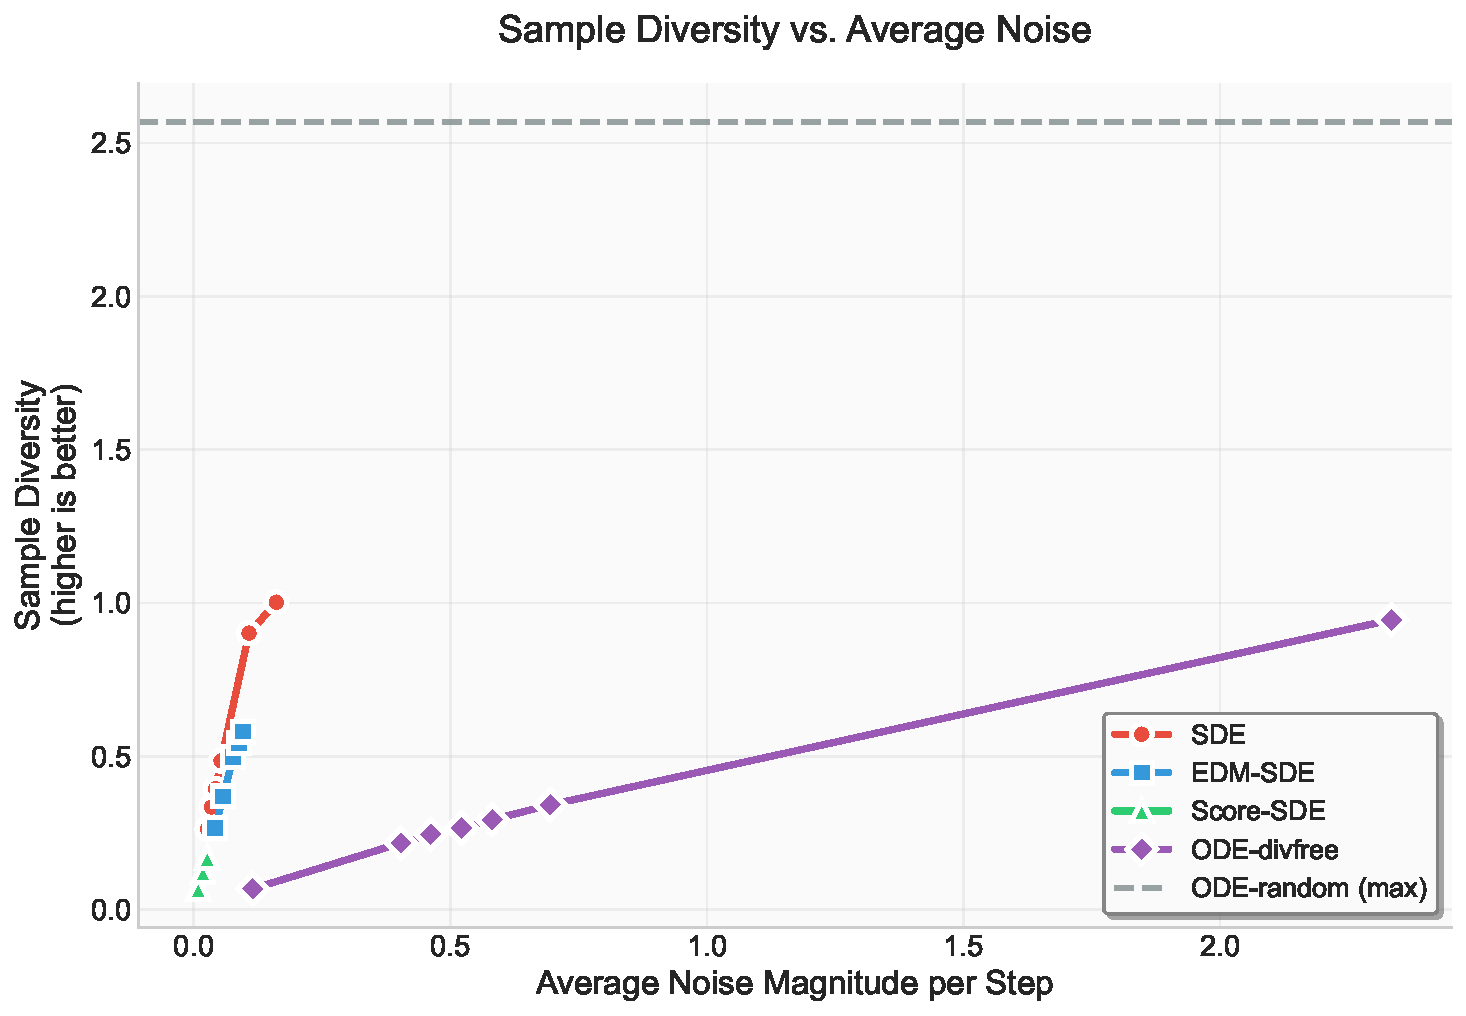
\includegraphics[width=\textwidth]{figures/noise_study_div.pdf}
    \caption{Sample diversity across increasing noise levels. Higher is better.}
    \label{fig:div-noise}
  \end{minipage}
  \hfill
  \begin{minipage}{0.48\textwidth}
    \centering
    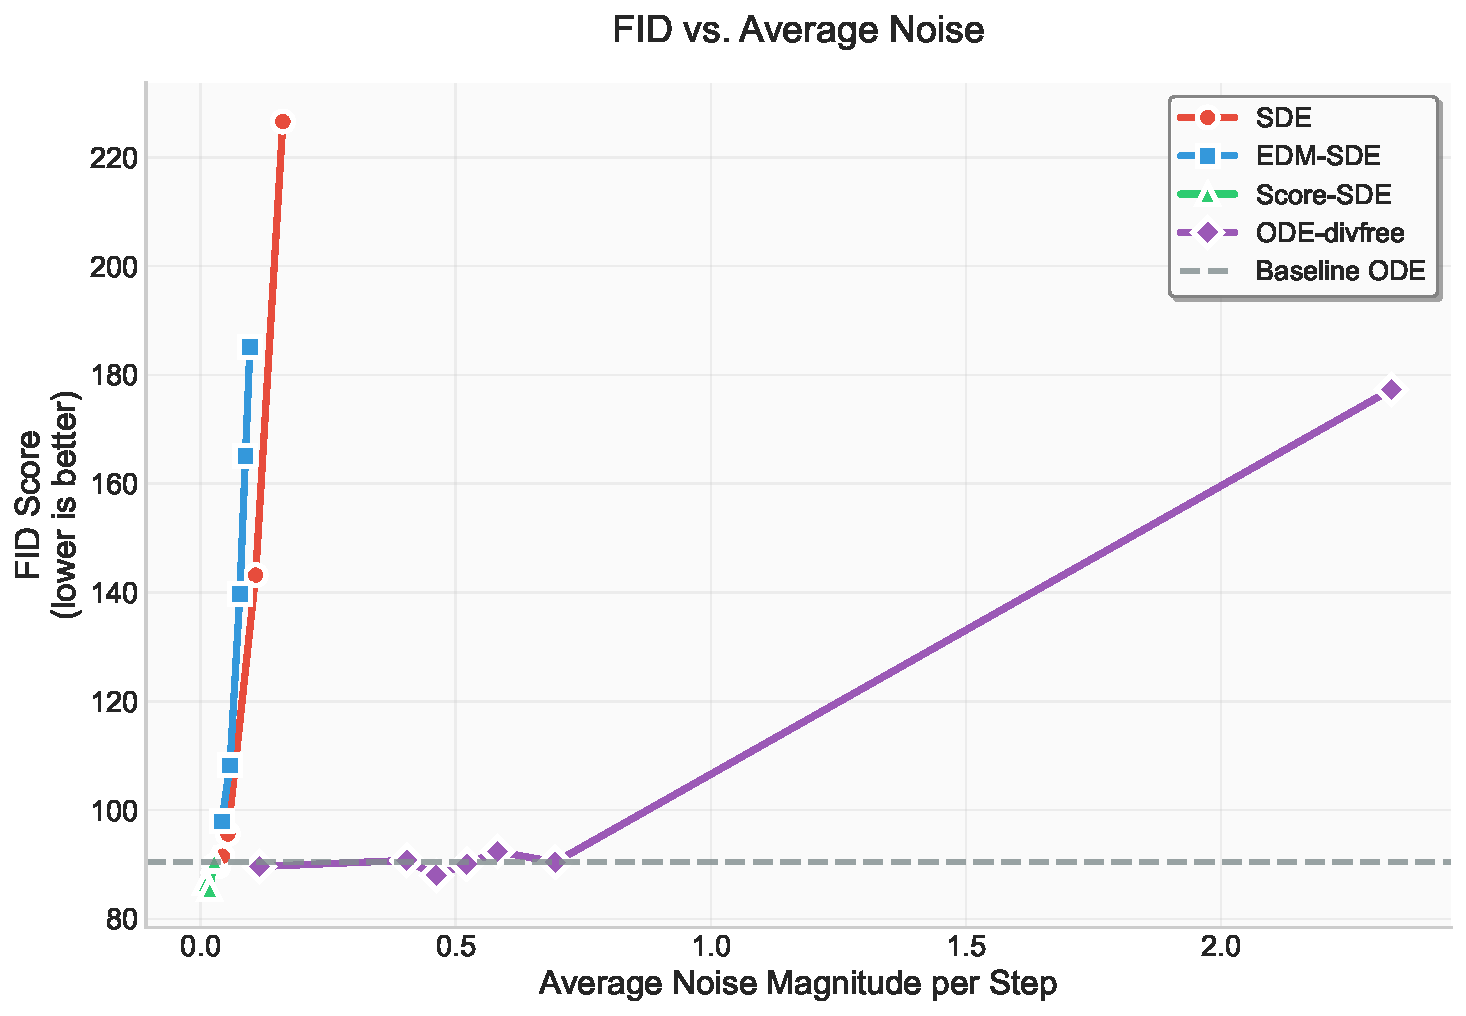
\includegraphics[width=\textwidth]{figures/noise_study_fid.pdf}
    \caption{FID across increasing noise levels. Lower is better.}
    \label{fig:fid-noise}
  \end{minipage}
\end{figure}

\begin{figure}[H]
  \centering
  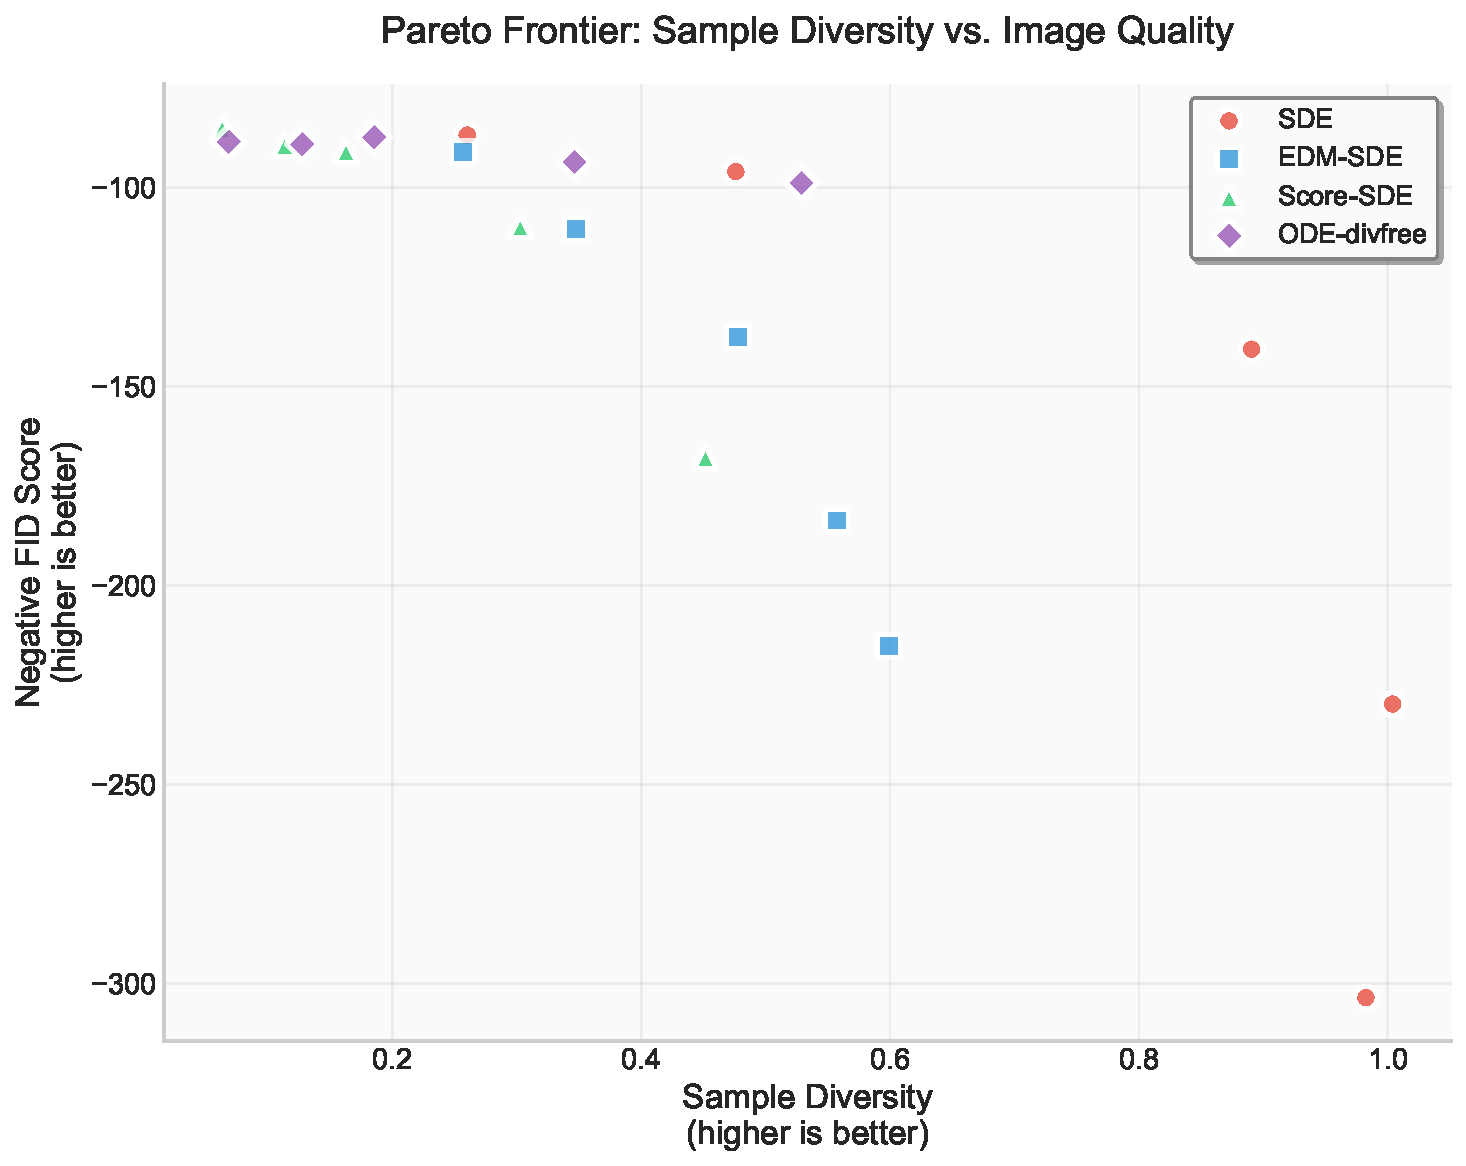
\includegraphics[width=0.7\linewidth]{figures/pareto_diversity_vs_fid.pdf}
  \caption{Pareto frontier analysis showing the trade-off between sample diversity and image quality (negative FID, where higher is better for both axes). Our divergence-free method achieves favorable positions on the frontier, maintaining high image quality while enabling substantial diversity gains compared to other stochastic sampling approaches.}
  \label{fig:pareto-fid}
\end{figure}

\paragraph{Results.}
As shown in the figures, our divergence-free ODE approach allows substantially higher levels of noise to be injected without degrading sample quality. Sample diversity increases smoothly with noise level (Fig.~\ref{fig:div-noise}), while FID remains stable across a wide noise range (Fig.~\ref{fig:fid-noise}). The Pareto frontier analysis (Fig.~\ref{fig:pareto-fid}) demonstrates that our method achieves superior trade-offs between diversity and quality compared to alternative stochastic approaches. In contrast, standard SDE sampling degrades rapidly as noise increases. EDM sampling performs better than the naïve SDE—consistent with its theoretical guarantee of preserving \(p_t(x)\) in expectation—but still deteriorates earlier than our method. Similar analysis for Inception Score shows comparable results (see Appendix). This suggests that satisfying the continuity equation per trajectory, as our approach does, offers stronger robustness to stochasticity during sampling.

\subsection{Sampling Algorithm}
Algorithm~\ref{alg:divergence-free-sampling} describes our divergence-free path exploration method. The key idea is to inject divergence-free perturbations during ODE integration while preserving the continuity equation.

\begin{algorithm}[H]
\caption{Divergence-Free Path Exploration Sampling}
\label{alg:divergence-free-sampling}
\begin{algorithmic}[1]
\Require Flow matching model $v_\theta$, initial noise $x_0 \sim \pi_{\text{ref}}$, noise scale $\lambda$, number of time steps $N$, step size $h = 1/N$
\Ensure Generated sample $x_1$
\State $x \leftarrow x_0$
\For{$i = 0$ to $N-1$}
    \State $t \leftarrow i \cdot h$
    \State $u_t \leftarrow v_\theta(x, t)$ \Comment{Learned velocity field}
    \State $s_t \leftarrow \nabla_x \log p_t(x)$ \Comment{Score function from stochastic interpolants}
    \State $\varepsilon \sim \mathcal{N}(0, I)$ \Comment{Sample Gaussian noise}
    \State $\hat{s}_t \leftarrow s_t / \|s_t\|$ \Comment{Normalize score direction}
    \State $w_t \leftarrow (I - \hat{s}_t \hat{s}_t^T) \varepsilon$ \Comment{Project noise orthogonal to score}
    \State $\tilde{u}_t \leftarrow u_t + \lambda w_t$ \Comment{Add divergence-free perturbation}
    \State $x \leftarrow x + h \cdot \tilde{u}_t$ \Comment{Euler step with perturbed velocity}
\EndFor
\State \Return $x$
\end{algorithmic}
\end{algorithm}

\subsection{Two-Stage Random Search and Divergence-Free Exploration}
Building on the observation that our divergence-free method can operate on preselected noise priors, we develop a two-stage algorithm that combines random search with path exploration. The approach first performs random search to broadly explore noise space, then applies divergence-free branching to exploit the best initial conditions. This mirrors reinforcement learning's exploration vs. exploitation tradeoff, where random search provides diverse exploration while divergence-free methods enable focused local search around promising noises.

\begin{algorithm}[H]
\caption{Two-Stage Random Search + Divergence-Free Exploration}
\label{alg:two-stage-sampling}
\begin{algorithmic}[1]
\Require Flow matching model $v_\theta$, verifier function $r(\cdot)$, compute budget $B$, number of top candidates $K$
\Ensure Top-$K$ generated samples
\State \textbf{Stage 1:} Perform random search sampling with budget $B$
\State $\{x_0^*\} \leftarrow$ Save initial noises for top-$K$ samples by verifier score $r(\cdot)$
\State \textbf{Stage 2:} Apply divergence-free ODE sampling using $\{x_0^*\}$ as initial conditions
\State \Return Top-$K$ samples from all divergence-free branches
\end{algorithmic}
\end{algorithm}

This design leverages a key insight from our diversity study: random search achieves high diversity since each sample is independent, whereas divergence-free sampling from the same initial noise has lower diversity but enables systematic local exploration. The two-stage combination captures the strengths of both approaches.


\section{Experiments}

\paragraph{Path Exploration.}
Our inference-time scaling methods primarily rely on path exploration, a strategy that generates multiple diverse trajectories from the same or similar initial conditions. Unlike random search which samples independently from the prior distribution, path exploration introduces controlled perturbations during the integration process to systematically explore the space of possible generation paths. This enables focused search around promising regions while maintaining the underlying model structure.

\subsection{ImageNet 256×256: Inference-Time Scaling with SiT-XL/2}

We demonstrate the effectiveness of our inference-time scaling approach on ImageNet 256×256 using the pretrained \textsc{SiT-XL/2} flow-matching model.

\subsubsection{Experimental Setup}

We compare five inference-time scaling methods across compute budgets of 1×, 2×, 4×, and 8×, where the compute factor corresponds to the number of parallel sampling branches. All methods start from the same baseline of generating 1,000 samples using the deterministic ODE sampler (1× compute). For scaled compute budgets, we generate multiple candidate samples and select the best ones according to different verifier functions.

We evaluate our divergence-free path exploration methods (ODE-divfree explore, RS → Divfree explore), Score SDE exploration, and SDE exploration as described in Section~4, along with Random Search (often termed Best-of-N)~\cite{ma2025diffits}, which generates multiple samples from different initial noise vectors and selects the top samples based on verifier score.

\subsubsection{Evaluation Metrics and Verifiers}

We evaluate performance using four metrics: FID (lower is better), Inception Score (higher is better), DINO Top-1 accuracy (higher is better), and DINO Top-5 accuracy (higher is better). Inception Score measures the quality and diversity of generated images based on a pretrained ImageNet classifier~\cite{salimans2016improved}. DINO scores evaluate semantic quality using self-supervised vision transformer features that capture richer visual representations~\cite{caron2021emerging}. FID computes the Fréchet distance between generated and real image feature distributions, providing a comprehensive measure of sample quality and diversity~\cite{heusel2017gans}. Each experiment uses two different verifier functions for sample selection: Inception Score-based scoring and DINO-based scoring.

\subsubsection{Results: Inception Score-Guided Scaling}

Figure~\ref{fig:inception-scaling} shows the results when using Inception Score as the verifier for sample selection. We report Inception Score and DINO Top-1 accuracy as the primary metrics, as these capture different aspects of sample quality.

\begin{figure}[H]
  \centering
  \begin{minipage}{0.48\textwidth}
    \centering
    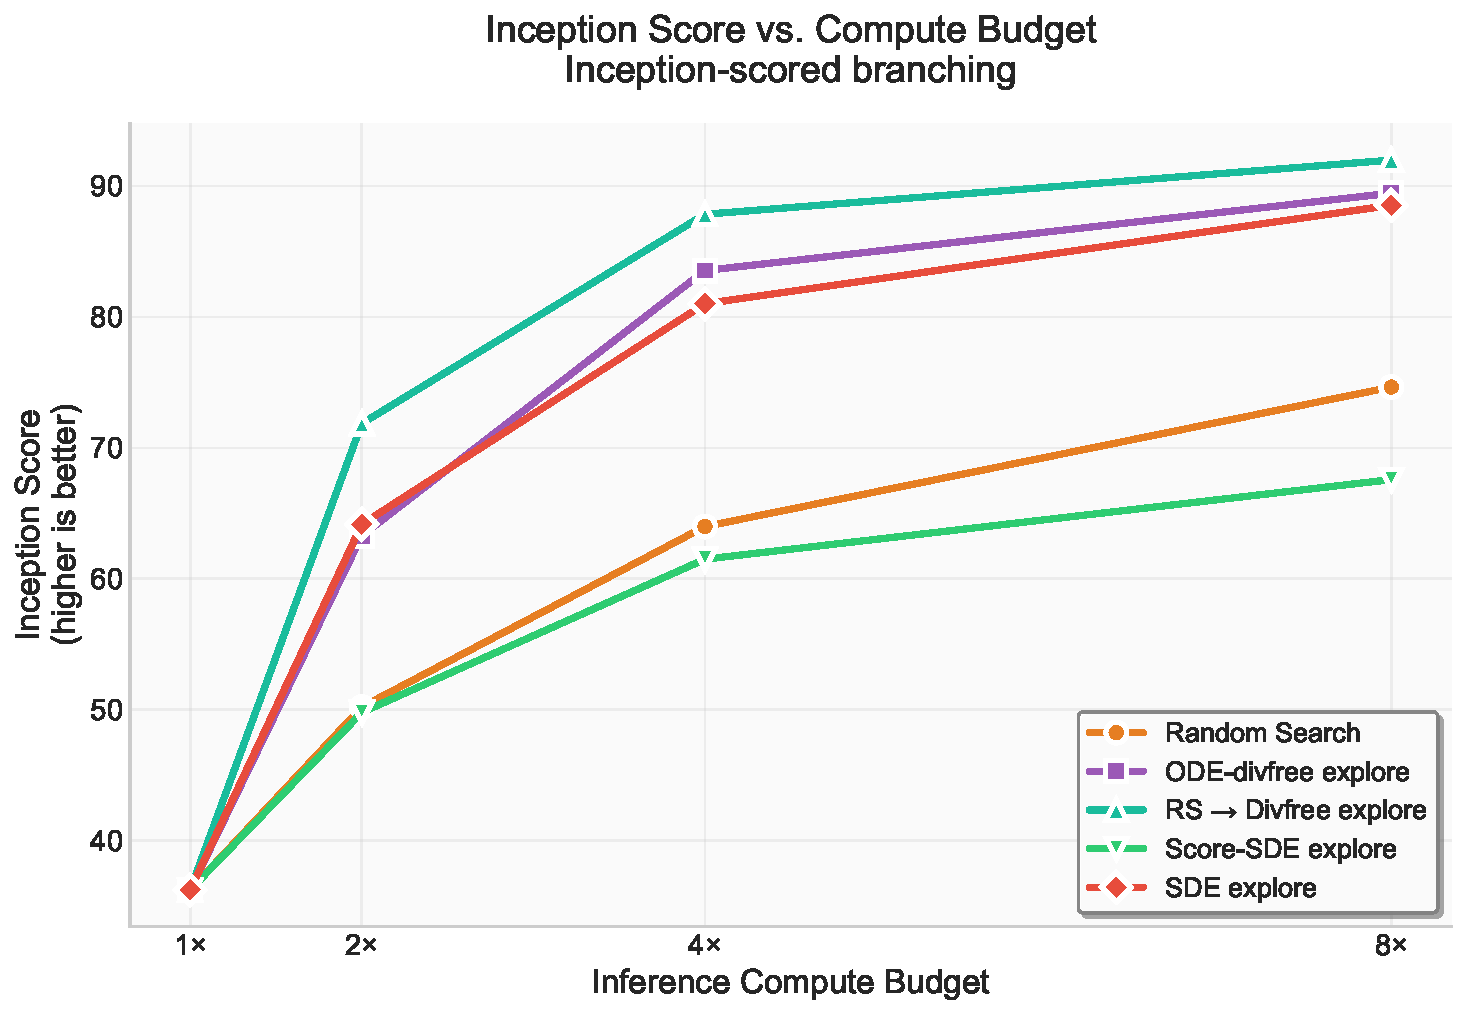
\includegraphics[width=\textwidth]{figures/scaling_inception_is.pdf}
  \end{minipage}
  \hfill
  \begin{minipage}{0.48\textwidth}
    \centering
    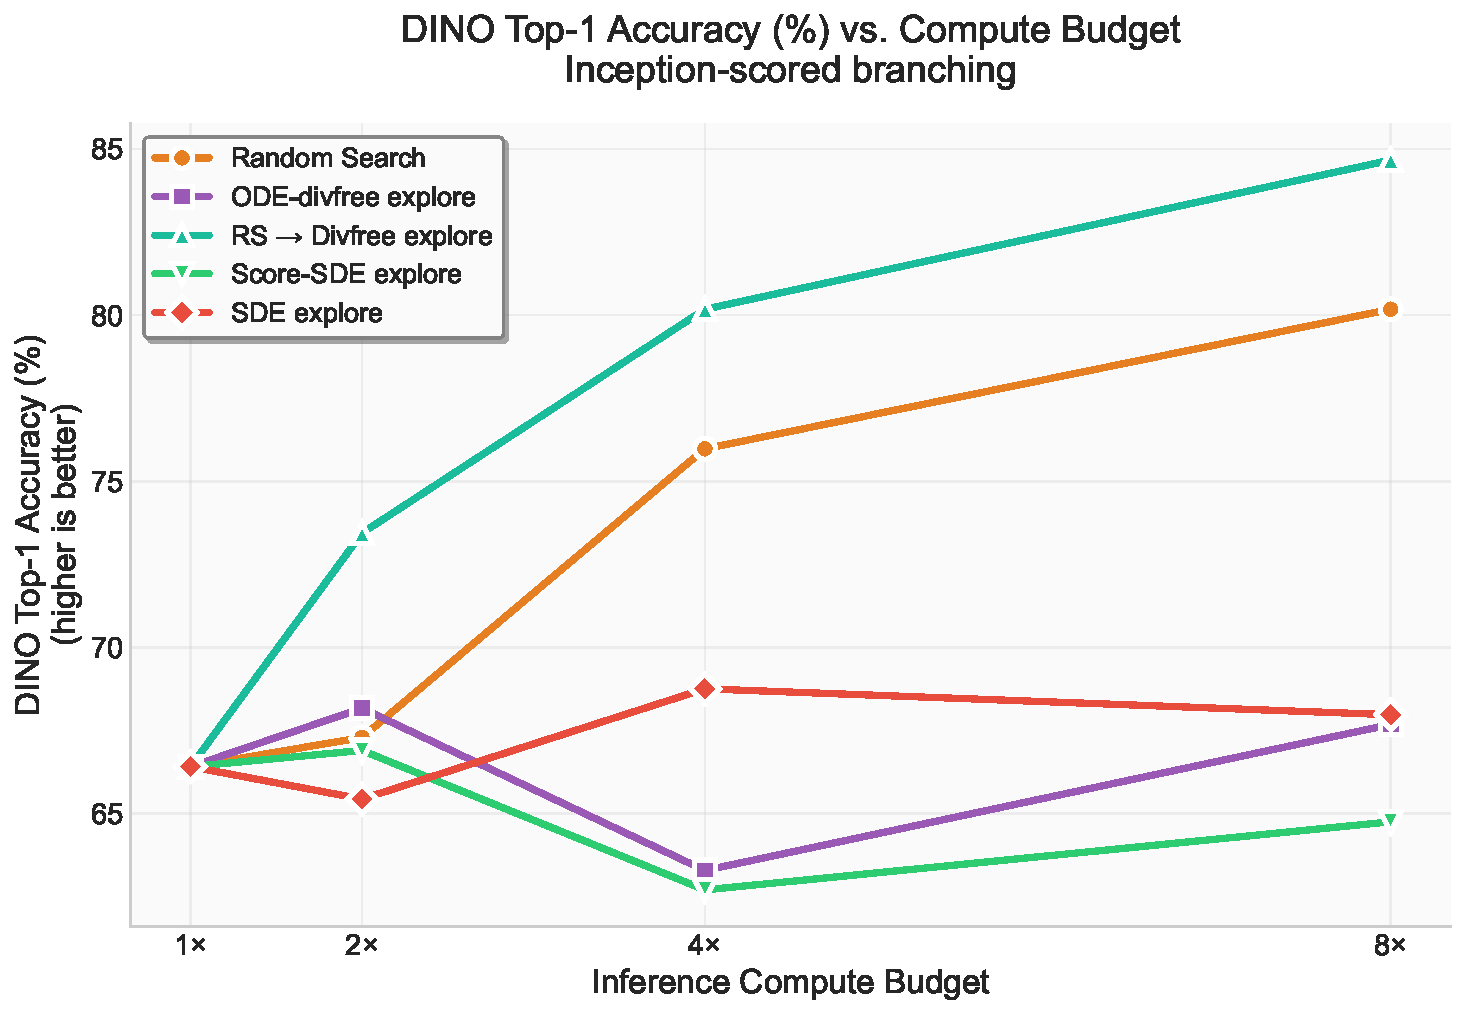
\includegraphics[width=\textwidth]{figures/scaling_inception_top1.pdf}
  \end{minipage}
  \caption{Inference-time scaling results using Inception Score-guided selection. Left: Inception Score vs. compute budget. Right: DINO Top-1 accuracy vs. compute budget.}
  \label{fig:inception-scaling}
\end{figure}

The RS → Divfree explore method demonstrates the strongest performance, achieving the highest Inception Scores at 4× and 8× compute budgets. This two-stage approach effectively combines the benefits of searching over initial conditions with path-space exploration. The ODE-divfree explore method shows steady improvement but is limited by starting from a single initial condition. Random search provides consistent but modest gains, while the SDE-based methods show more variable performance.

\subsubsection{Results: DINO-Guided Scaling}

Figure~\ref{fig:dino-scaling} presents results when using DINO-based scoring for sample selection. We focus on FID, Inception Score, and DINO Top-1 accuracy as key performance indicators.

\begin{figure}[H]
  \centering
  \begin{minipage}{0.32\textwidth}
    \centering
    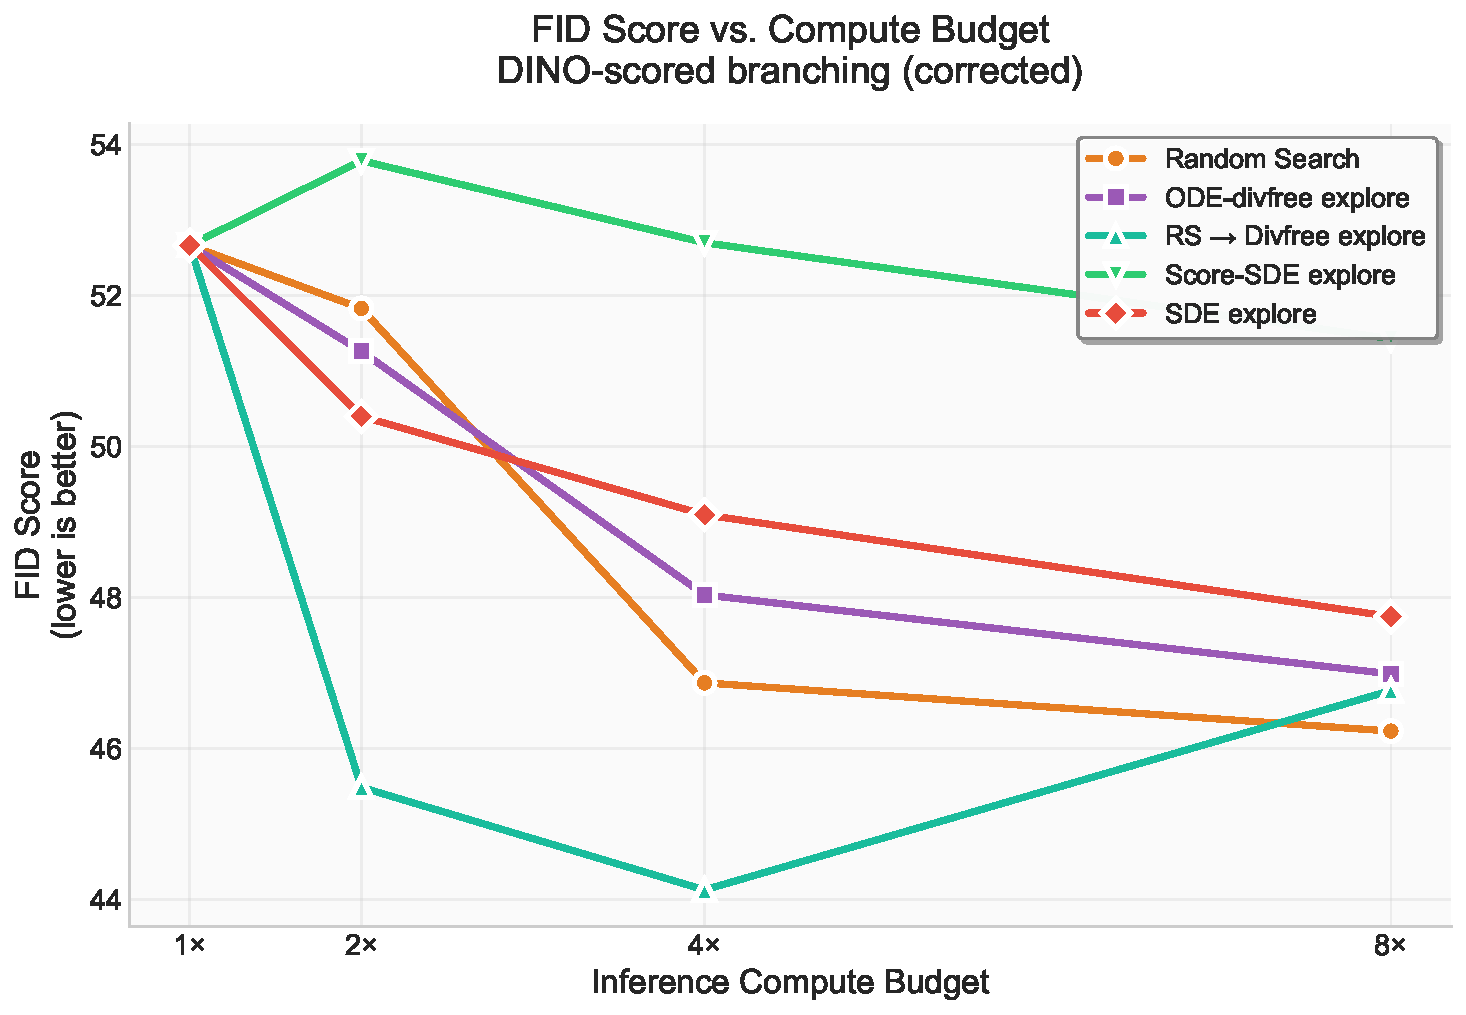
\includegraphics[width=\textwidth]{figures/scaling_dino_fid.pdf}
  \end{minipage}
  \hfill
  \begin{minipage}{0.32\textwidth}
    \centering
    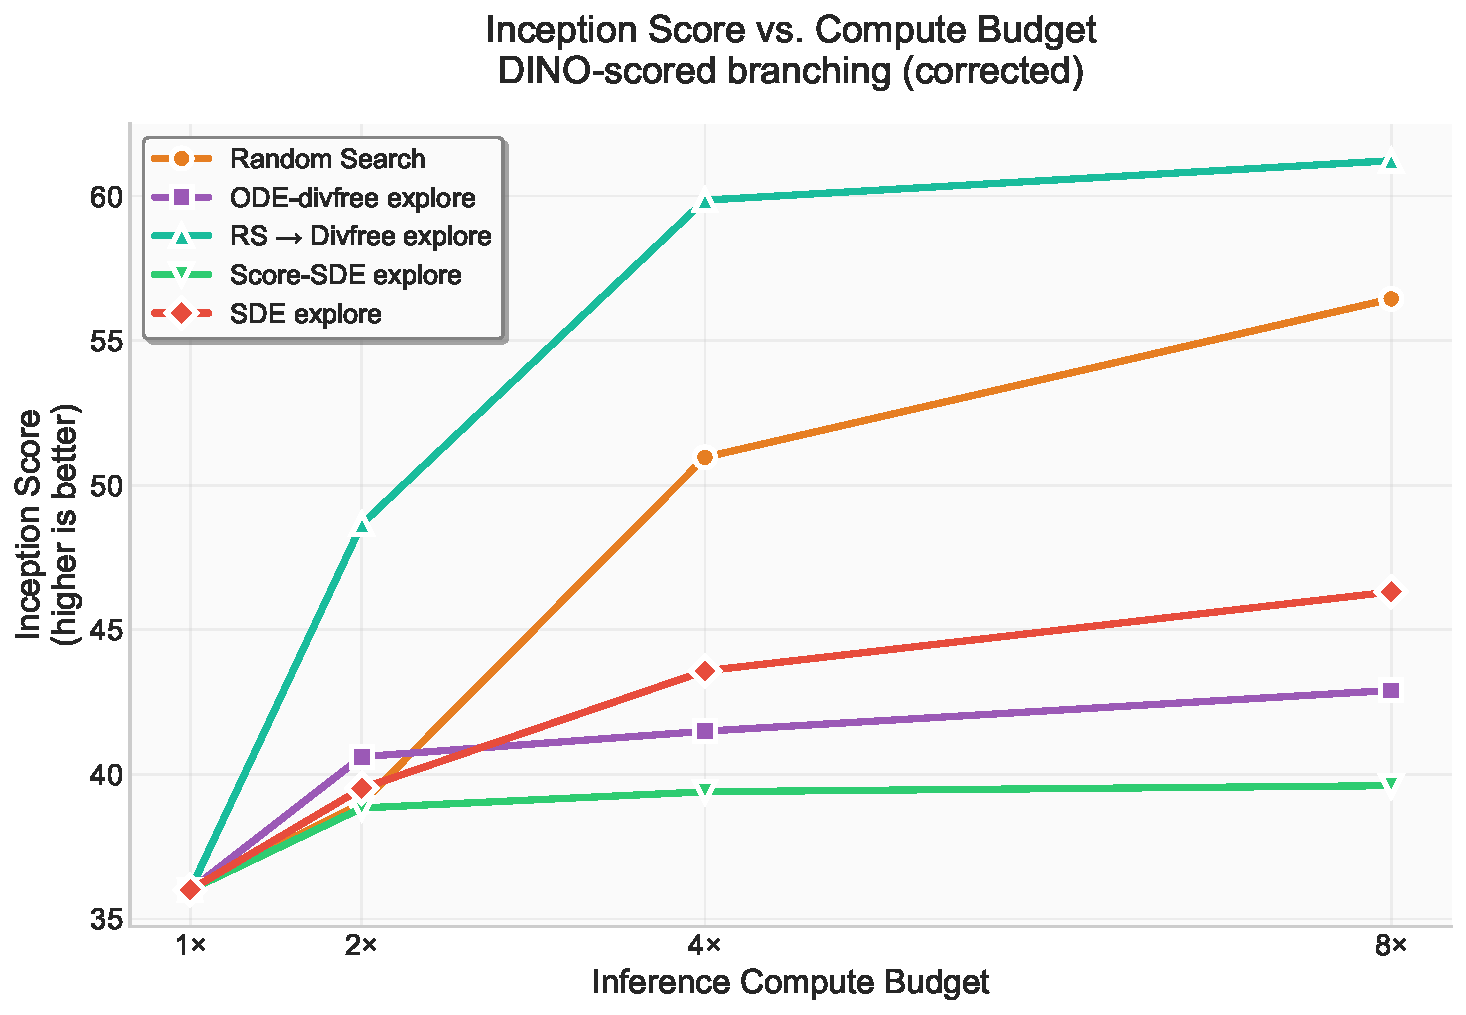
\includegraphics[width=\textwidth]{figures/scaling_dino_is.pdf}
  \end{minipage}
  \hfill
  \begin{minipage}{0.32\textwidth}
    \centering
    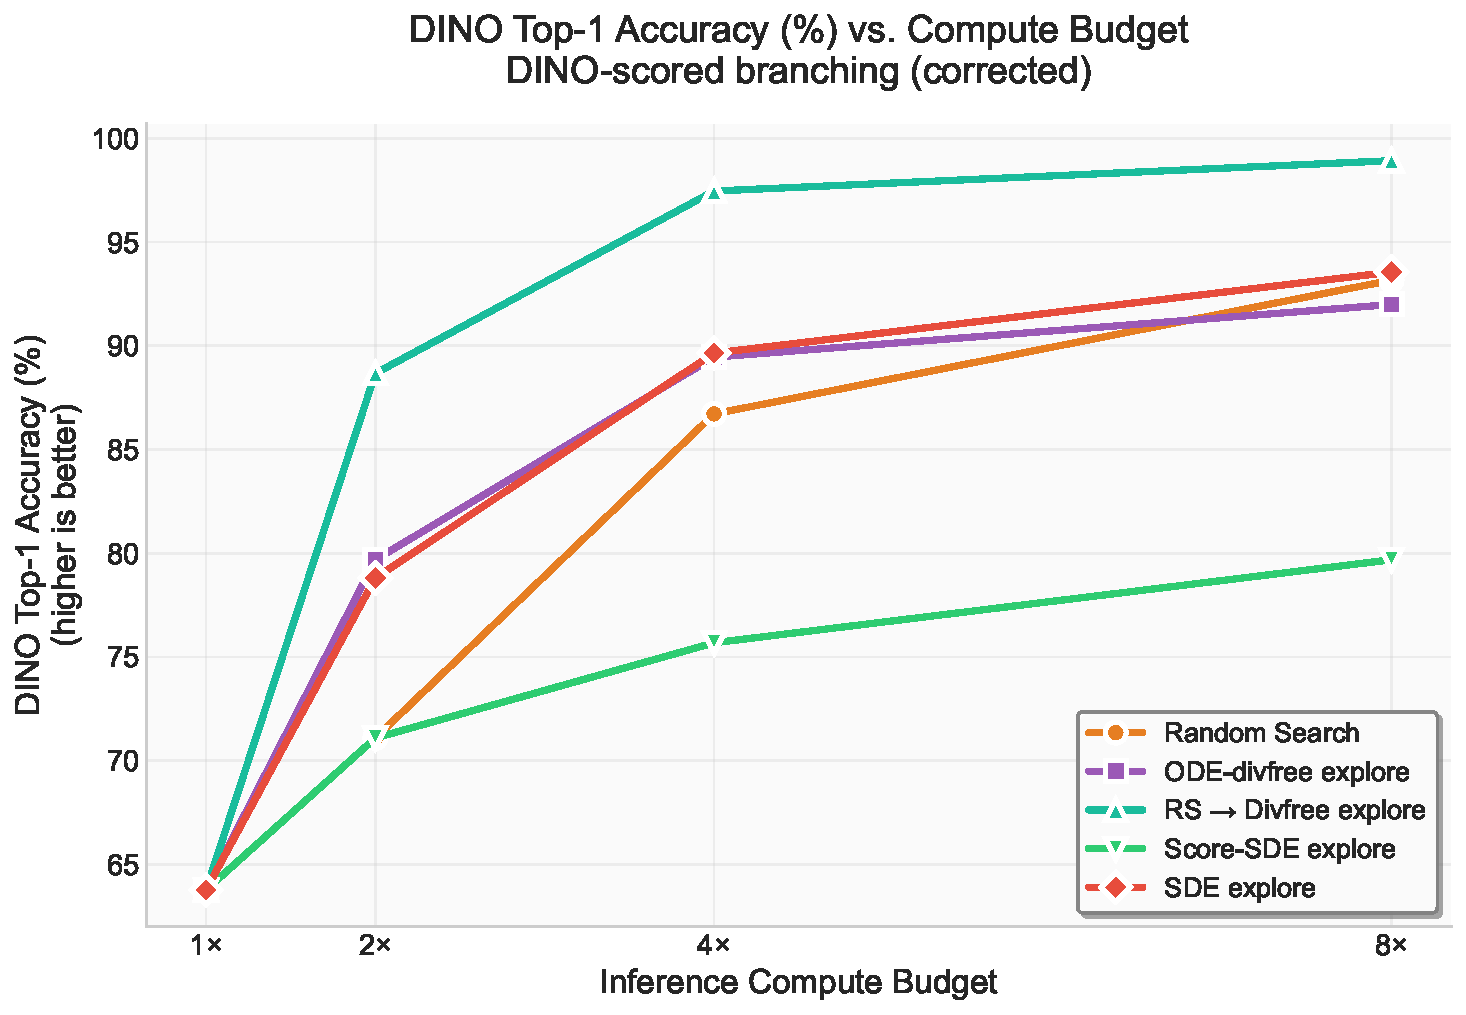
\includegraphics[width=\textwidth]{figures/scaling_dino_top1.pdf}
  \end{minipage}
  \caption{Inference-time scaling results using DINO-guided selection. Left: FID vs. compute budget. Center: Inception Score vs. compute budget. Right: DINO Top-1 accuracy vs. compute budget.}
  \label{fig:dino-scaling}
\end{figure}

Under DINO-guided selection, the RS → Divfree explore method again shows superior performance, achieving the best FID scores and DINO Top-1 accuracy at higher compute budgets. Notably, DINO-guided selection produces more substantial improvements in DINO Top-1 accuracy compared to Inception-guided selection, demonstrating the importance of verifier-method alignment. The ODE-divfree explore method shows consistent improvement across all metrics, while random search and SDE methods provide more modest gains.

\subsection{FoldFlow: Protein Design}

We evaluate our inference-time scaling methods on protein structure generation using the pretrained FoldFlow model~\cite{wu2024foldflow}. FoldFlow is a continuous normalizing flow model that generates protein backbone structures by learning the conditional distribution of protein coordinates given sequence information. This provides an important validation of our approach in a different scientific domain with distinct evaluation metrics.

\subsubsection{Experimental Setup}

We apply the same inference-time scaling methods from our ImageNet experiments to protein generation: Random Search (Best-of-N), ODE-divfree explore, SDE path exploration, and Random Search → Divfree explore (two-stage). We evaluate across compute budgets of 1×, 2×, 4×, and 8× using 64 protein samples per configuration. All methods are compared against the standard deterministic ODE sampling baseline (1× compute).

The evaluation metric is designability, computed using the self-consistency TM-score~\cite{wu2024foldflow}. This metric compares refolded proteins (using ProteinMPNN~\cite{dauparas2022protein} and ESMFold~\cite{lin2022language}) with the original generated structures. Higher TM-scores indicate better structural quality and biological plausibility, with scores ranging from 0 to 1 where values above 0.8 typically indicate high-quality protein structures.

\subsubsection{Results}

Figure~\ref{fig:protein-scaling} shows the mean TM-scores across different compute budgets for each inference-time scaling method.

\begin{figure}[H]
  \centering
  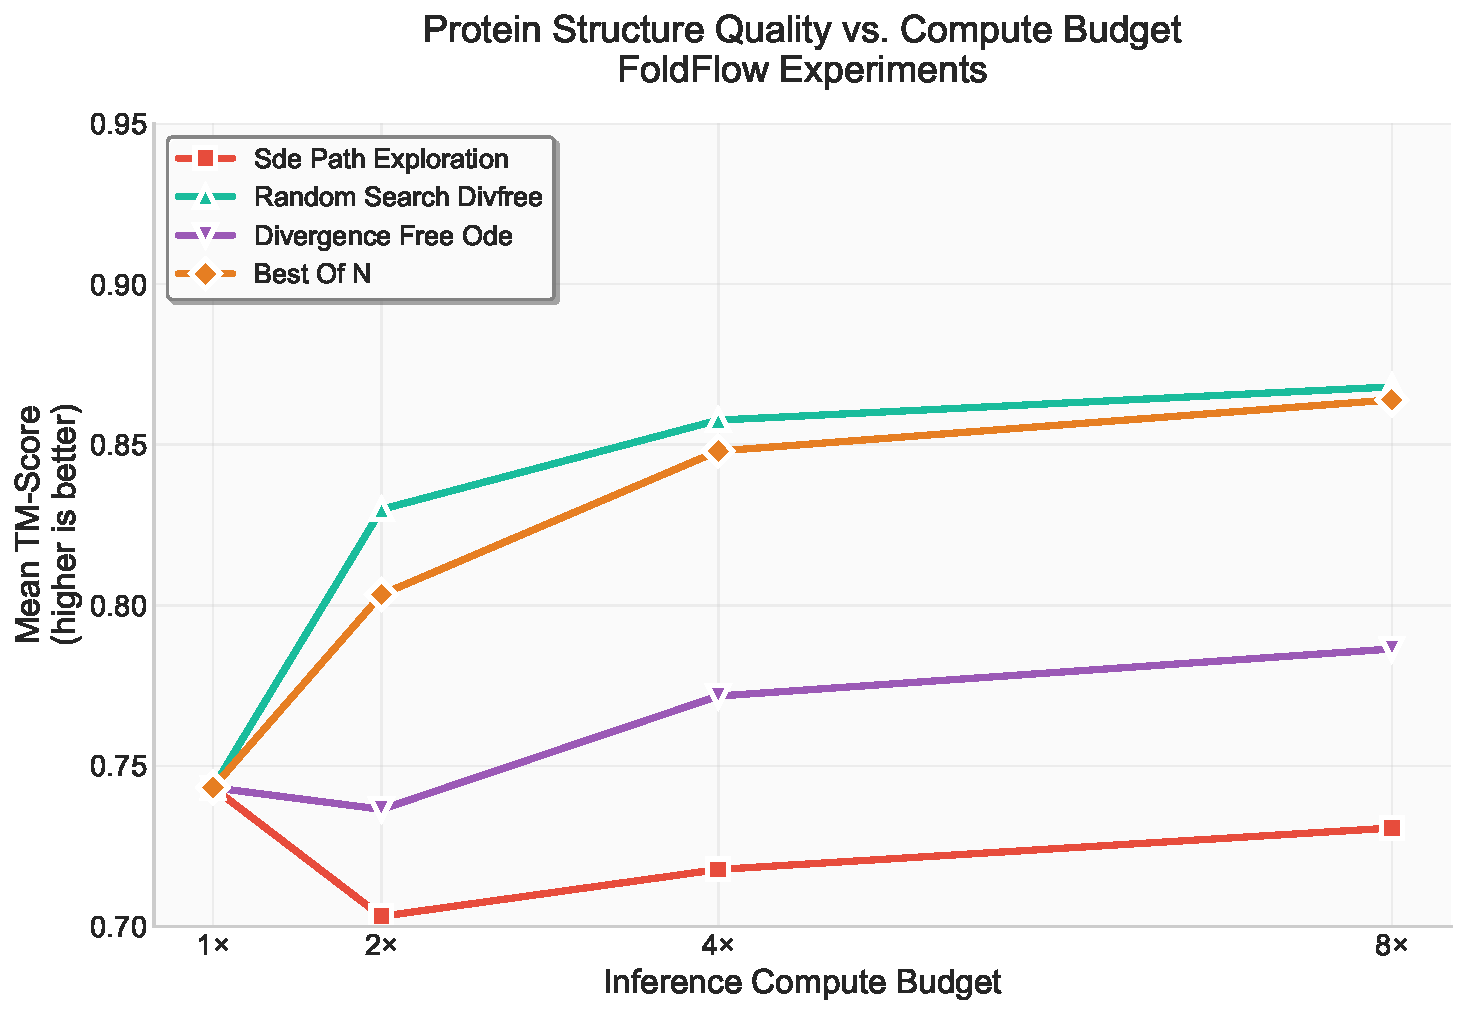
\includegraphics[width=0.8\linewidth]{figures/protein_scaling_tm_score.pdf}
  \caption{Protein structure quality (TM-score) vs. compute budget for FoldFlow experiments. All methods start from the same baseline (standard ODE sampling at 1× compute) and show how additional inference compute improves protein designability.}
  \label{fig:protein-scaling}
\end{figure}

The results demonstrate clear benefits of inference-time scaling for protein generation:

\paragraph{Two-Stage Superiority.} The Random Search → Divfree explore method achieves the highest TM-scores across all compute budgets, reaching 0.868 at 8× compute compared to the 0.743 baseline. This represents a substantial improvement in protein quality, with TM-scores consistently above 0.82 even at 2× compute.

\paragraph{Best-of-N Effectiveness.} Random Search (Best-of-N) shows strong performance, achieving 0.864 at 8× compute. This suggests that searching over initial conditions is particularly effective for protein generation, likely due to the discrete nature of protein sequence-structure relationships.

\paragraph{Path Exploration Benefits.} ODE-divfree explore shows steady improvement from 0.743 to 0.786 at 8× compute, demonstrating that divergence-free perturbations can improve protein quality even when starting from a single initial condition. SDE path exploration shows more modest gains but still provides consistent improvements over the baseline.

\paragraph{Compute-Quality Tradeoffs.} All methods demonstrate favorable compute-quality tradeoffs, with the most substantial improvements occurring at 2× and 4× compute budgets. The diminishing returns at 8× compute suggest practical limits to inference-time scaling, but even modest compute increases yield meaningful improvements in protein designability.

\subsubsection{Analysis}

The strong performance of our methods on protein generation validates the general applicability of inference-time scaling beyond image generation. The particularly strong showing of Random Search methods suggests that the discrete nature of protein sequences may make initial condition search especially valuable. The consistent improvements from divergence-free path exploration demonstrate that our method successfully transfers to scientific applications with different evaluation criteria and domain-specific constraints.

These results establish inference-time scaling as a promising approach for improving protein design quality without requiring model retraining, opening possibilities for enhanced drug discovery and protein engineering applications.

\section{Conclusion}

We have introduced the first comprehensive framework for inference-time scaling in flow matching models, addressing a critical gap in continuous-time generative modeling. Our approach preserves the mathematical foundations of flow matching while enabling principled exploration of alternative generation trajectories through divergence-free velocity perturbations.

\textbf{Key Achievements:} Our theoretical analysis proves that divergence-free perturbations maintain the continuity equation at the trajectory level, providing stronger guarantees than methods that preserve distributions only in expectation. This mathematical rigor enables robust performance across diverse noise levels and ensures compatibility with the linear interpolation paths that define flow matching. Our experimental validation demonstrates substantial improvements across two distinct domains: ImageNet image generation and protein structure design, with our two-stage approach consistently achieving the best performance.

\textbf{Methodological Insights:} Our work reveals complementary strengths of different scaling strategies. Random search provides broad exploration particularly valuable for discrete relationships (e.g., protein sequence-structure mappings), while divergence-free path exploration enables focused exploitation around promising regions. The two-stage combination captures benefits of both approaches, suggesting that inference-time scaling benefits from balancing exploration and exploitation.

\textbf{Practical Impact:} The training-free nature of our approach makes it immediately applicable to existing flow matching models across domains. For protein design, improvements from 0.743 to 0.868 TM-score represent meaningful advances in structural quality with implications for drug discovery and protein engineering. For image generation, our method provides a scalable path to higher quality samples without architectural modifications or retraining.

\textbf{Limitations and Future Work:} While our approach shows diminishing returns at higher compute budgets (8×), suggesting practical limits to inference-time scaling, even modest compute increases (2×-4×) yield substantial quality improvements. Future work could explore adaptive scaling strategies that optimize compute allocation based on sample complexity, integration with more sophisticated verifiers for domain-specific applications, and extension to other continuous-time generative models beyond flow matching.

\textbf{Broader Implications:} Our work positions inference-time scaling as a fundamental capability for continuous generative models, complementing training-time scaling. As generative models become increasingly important for scientific discovery and creative applications, the ability to trade computational resources for sample quality at inference time provides practitioners with valuable flexibility. This paradigm shift from "one model, one quality level" to "adjustable quality through inference compute" opens new possibilities for interactive applications, quality-critical deployments, and resource-constrained scenarios.

Looking forward, we envision inference-time scaling becoming a standard tool in the continuous generative modeling toolkit, enabling researchers and practitioners to extract maximum value from trained models while adapting to diverse quality requirements and computational constraints.

%%%%% References
\bibliographystyle{apalike}
\bibliography{main}

%%%%%%%%%%%%%%%%%%%%%%%%%%%%%%%%%%%%%%%%%%%%%%%%%%%%%%%%%%%%

\appendix

\section{Additional Experimental Results}

This appendix contains supplementary figures and detailed results that support the main findings presented in the paper.

\subsection{Complete Noise and Diversity Study Results}

\begin{figure}[H]
  \centering
  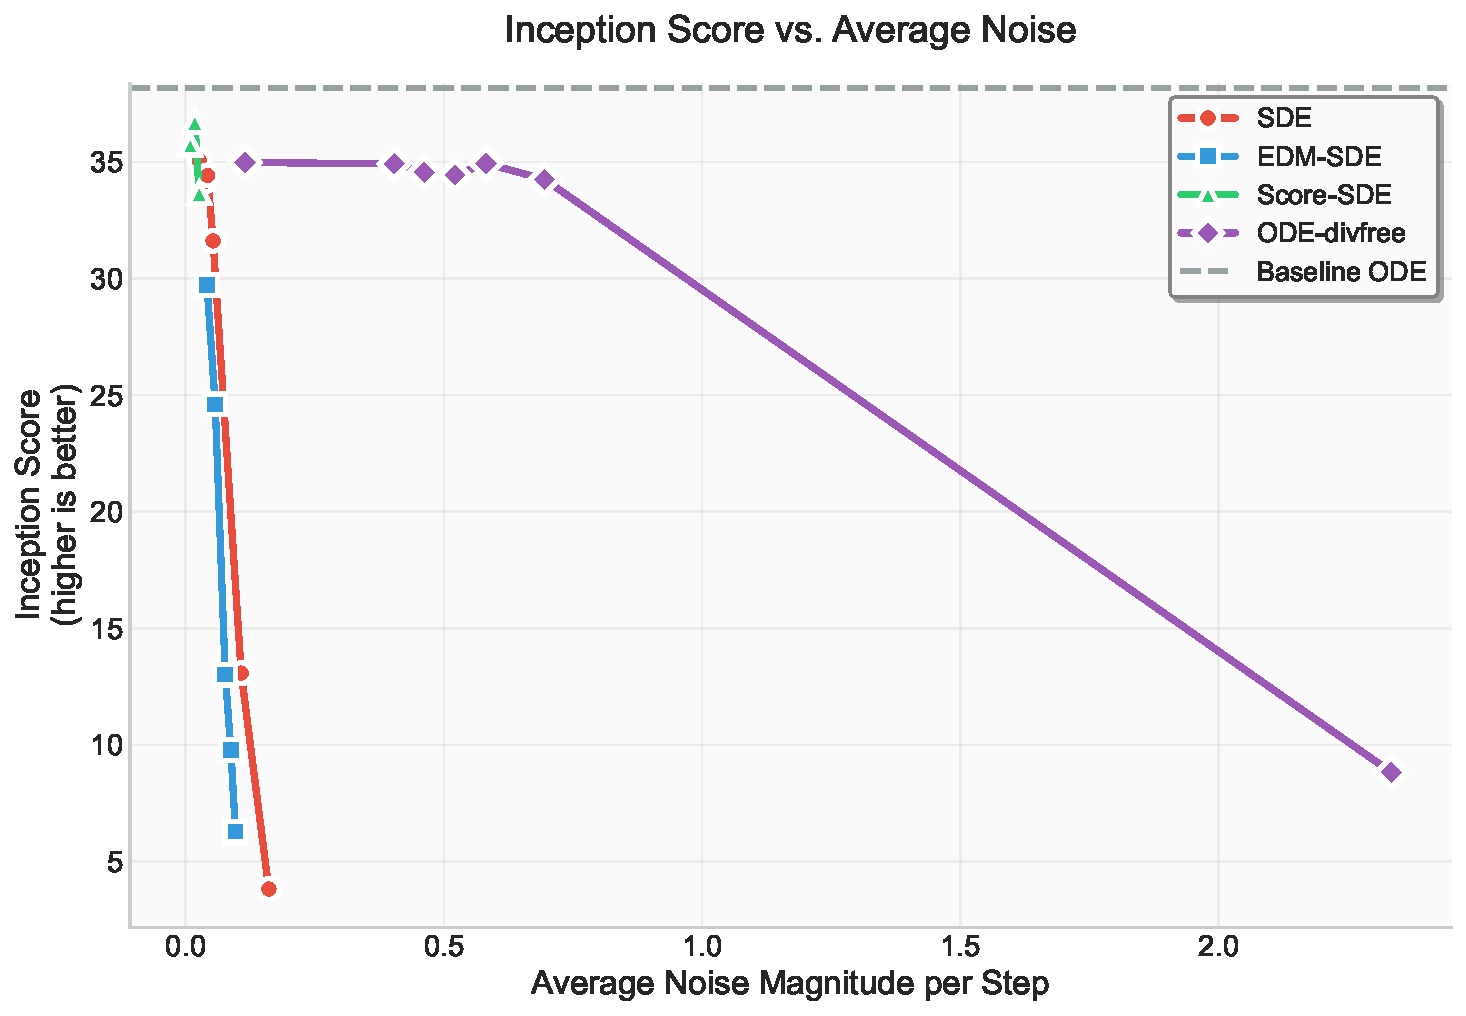
\includegraphics[width=0.7\linewidth]{figures/noise_study_is.pdf}
  \caption{Inception Scores across increasing noise levels. Higher is better. This complements the diversity and FID analysis shown in the main text, demonstrating similar robustness patterns for our divergence-free method.}
  \label{fig:is-noise}
\end{figure}

\begin{figure}[H]
  \centering
  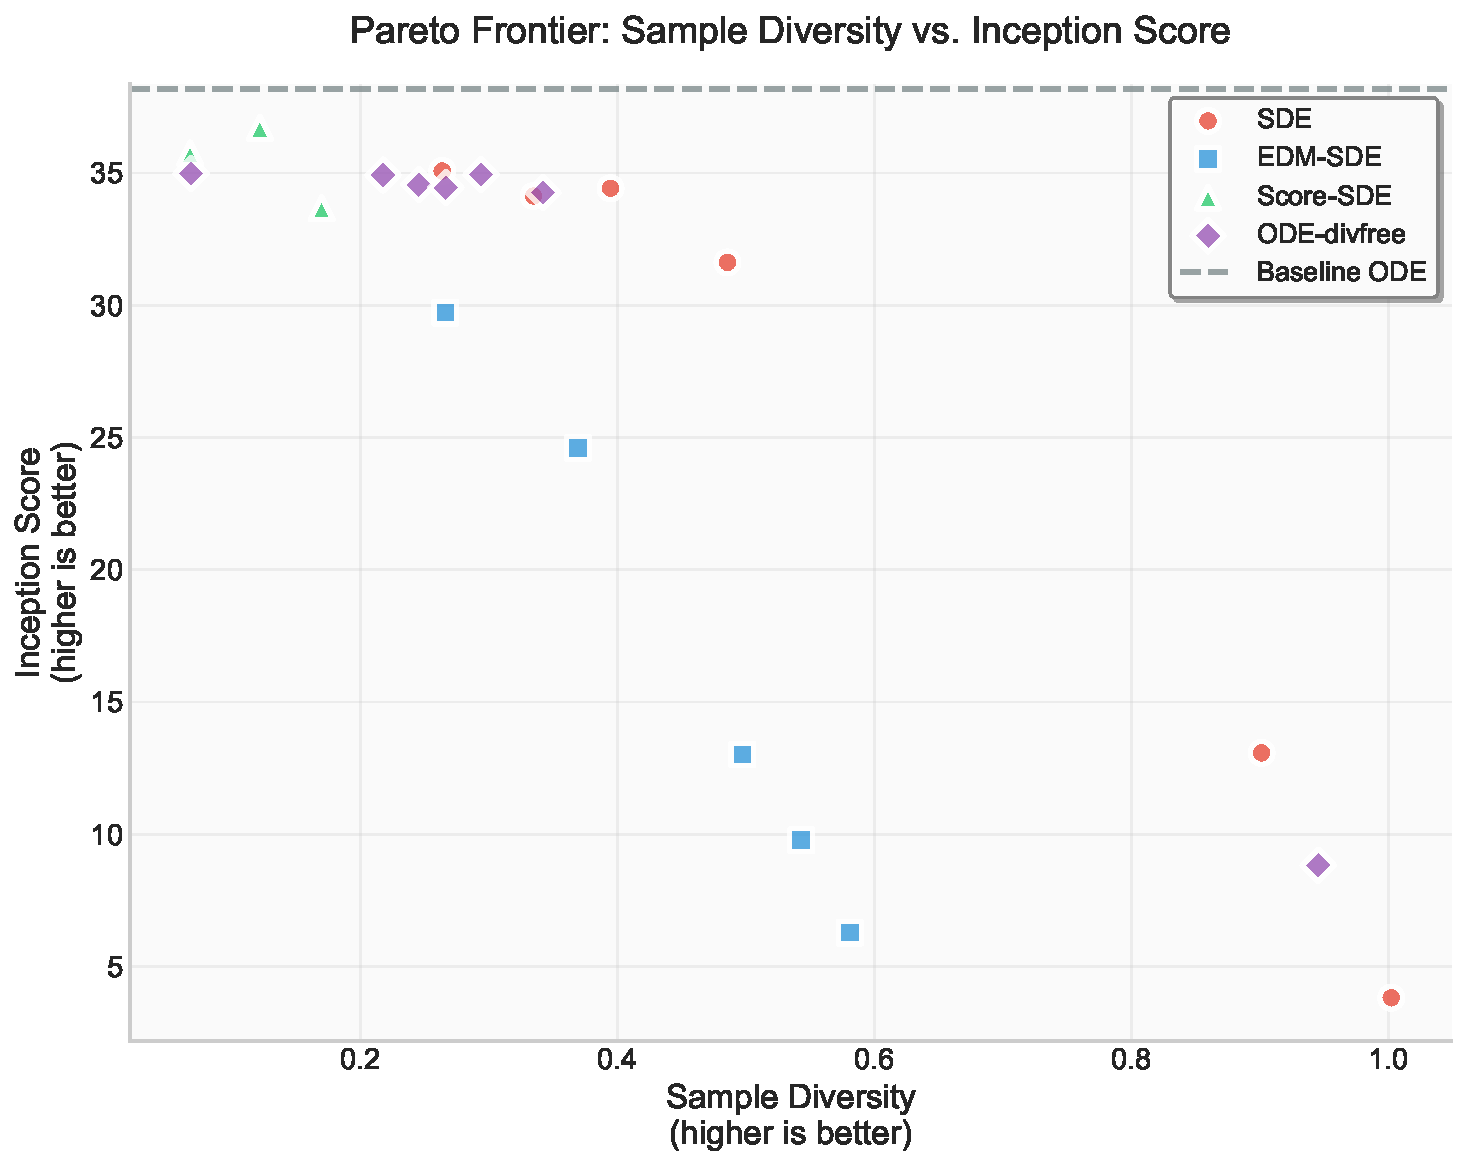
\includegraphics[width=0.7\linewidth]{figures/pareto_diversity_vs_inception.pdf}
  \caption{Pareto frontier analysis showing the trade-off between sample diversity and Inception Score (higher is better for both axes). This complements the FID-based Pareto analysis in the main text.}
  \label{fig:pareto-inception}
\end{figure}

\subsection{Complete Inference-Time Scaling Results}

\subsubsection{Inception Score-Guided Scaling (All Metrics)}

\begin{figure}[H]
  \centering
  \begin{minipage}{0.48\textwidth}
    \centering
    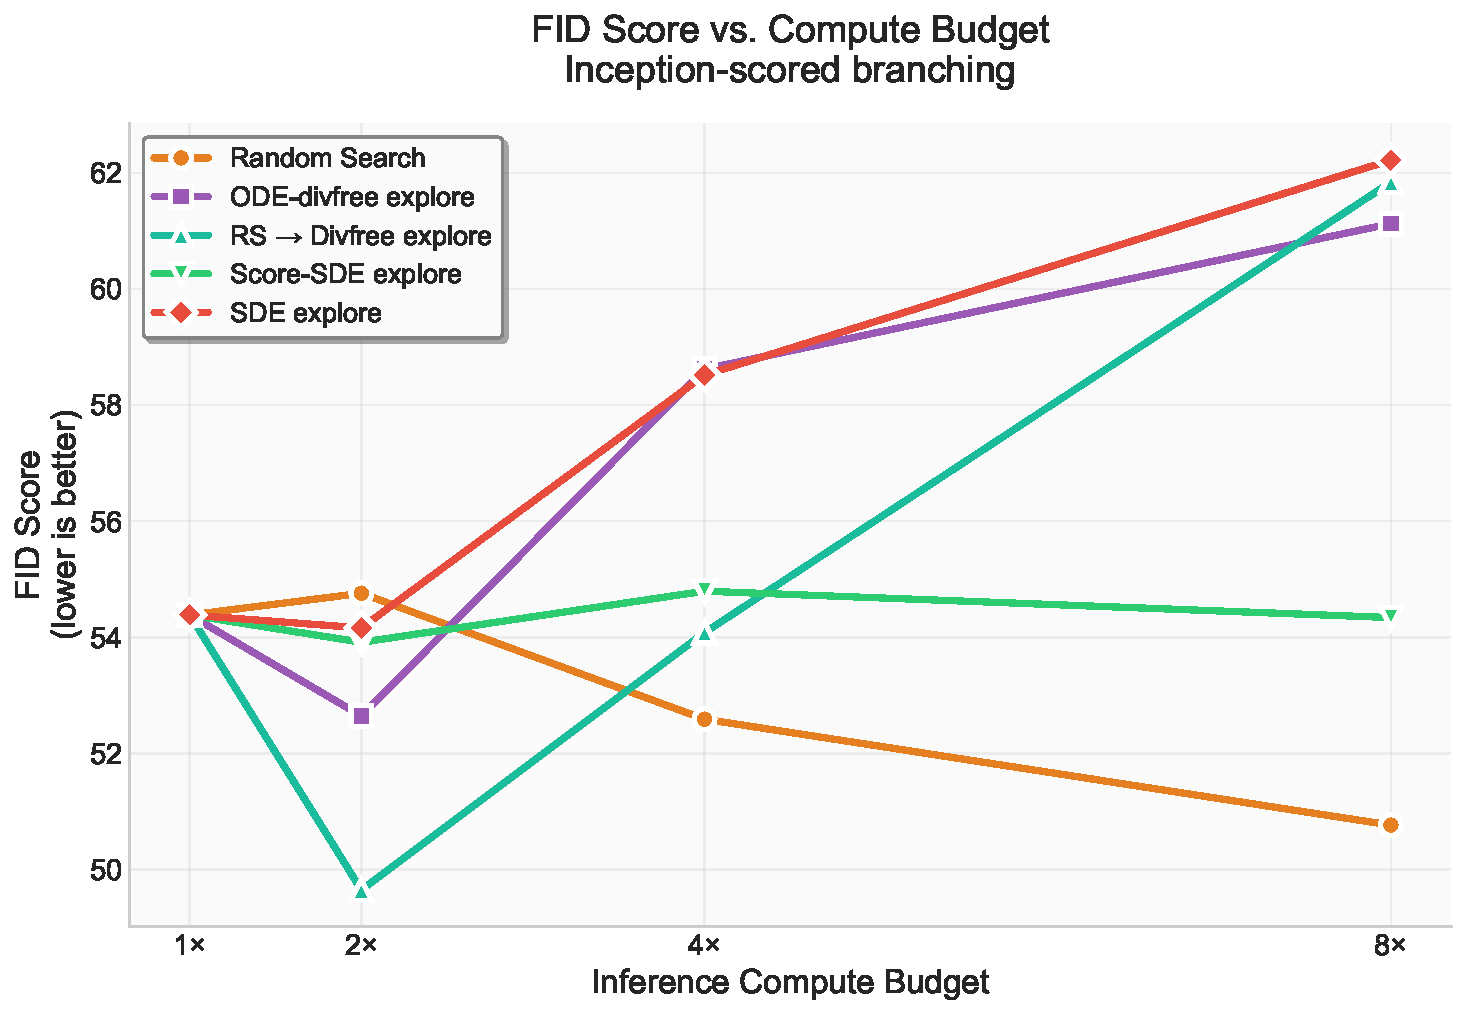
\includegraphics[width=\textwidth]{figures/scaling_inception_fid.pdf}
  \end{minipage}
  \hfill
  \begin{minipage}{0.48\textwidth}
    \centering
    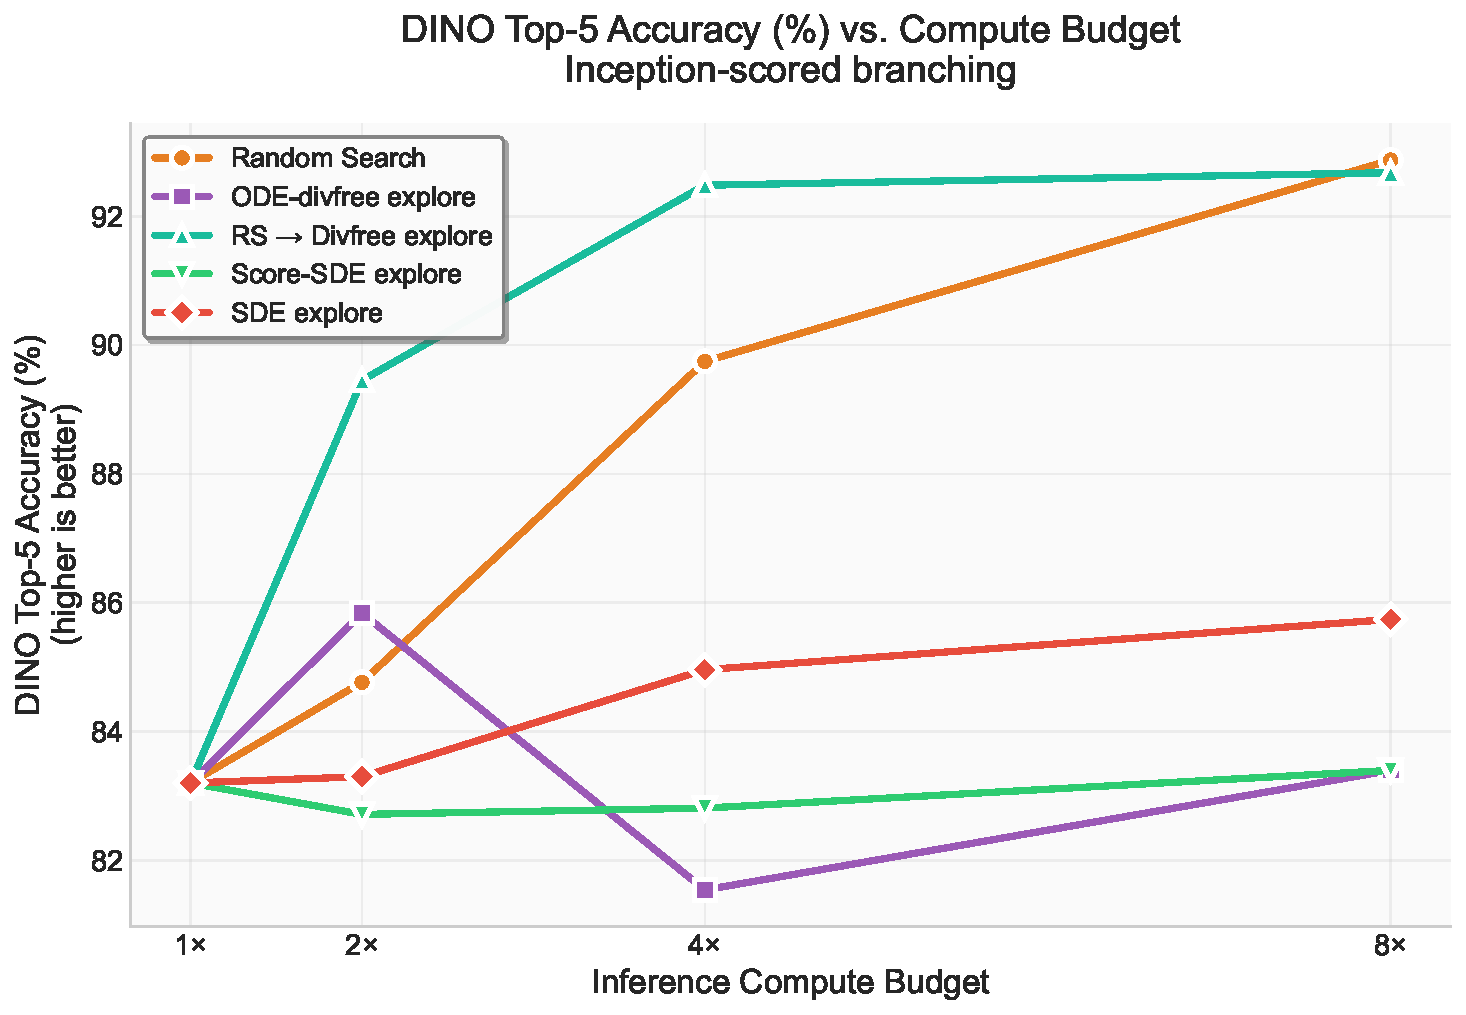
\includegraphics[width=\textwidth]{figures/scaling_inception_top5.pdf}
  \end{minipage}
  \caption{Additional Inception Score-guided scaling results. Left: FID vs. compute budget. Right: DINO Top-5 accuracy vs. compute budget.}
  \label{fig:inception-scaling-complete}
\end{figure}

\subsubsection{DINO-Guided Scaling (All Metrics)}

\begin{figure}[H]
  \centering
  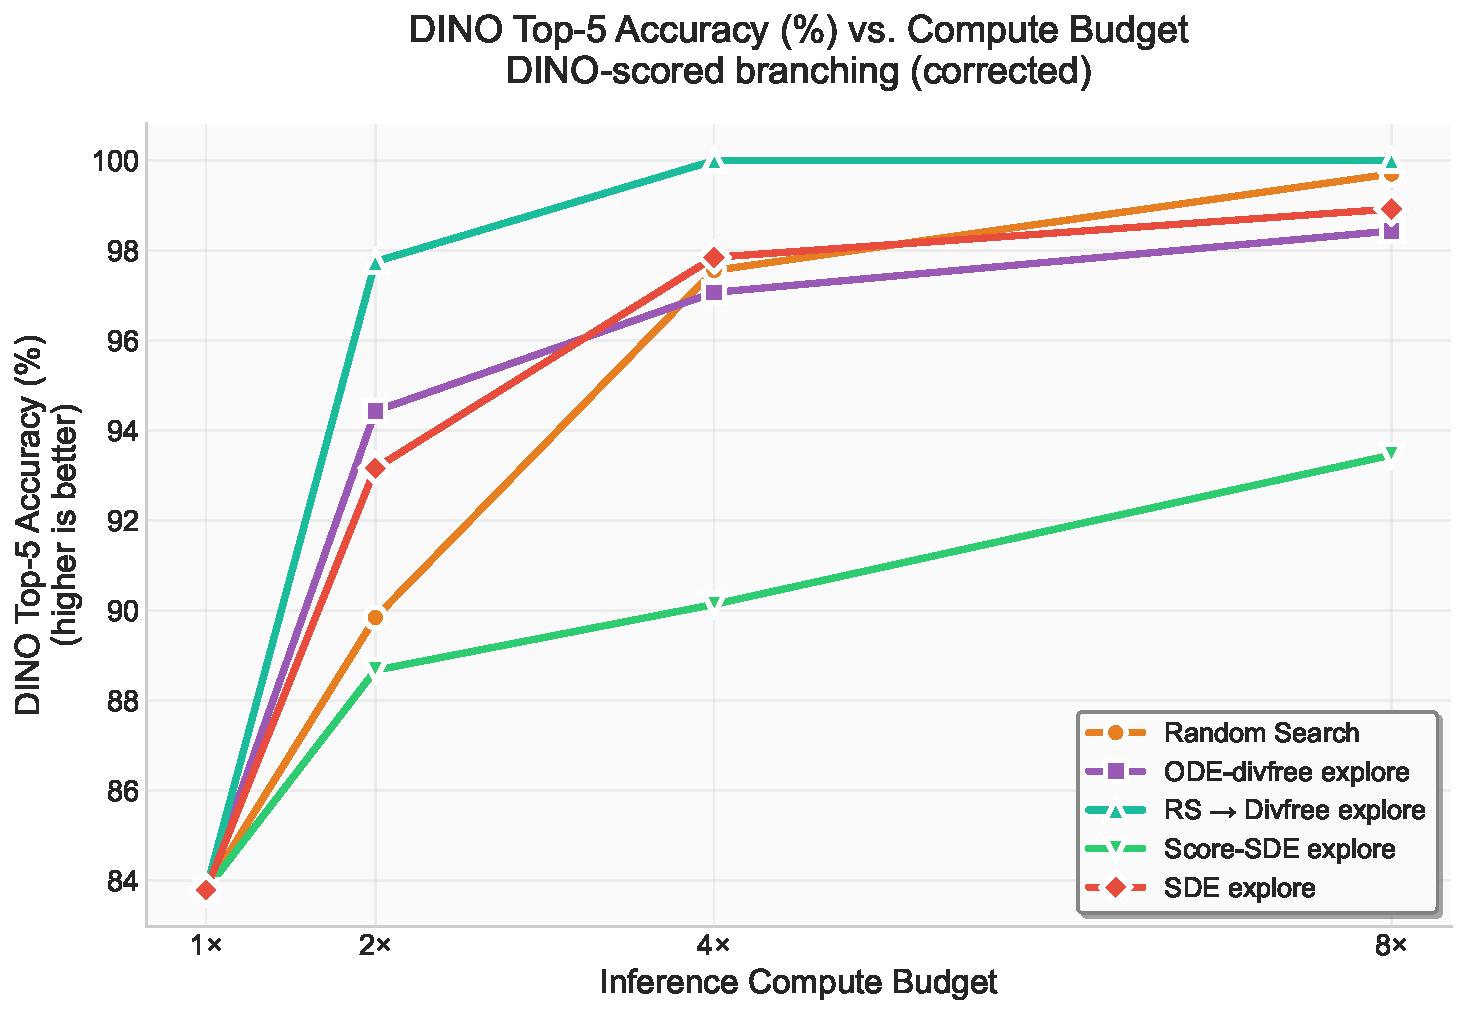
\includegraphics[width=0.48\textwidth]{figures/scaling_dino_top5.pdf}
  \caption{DINO Top-5 accuracy vs. compute budget for DINO-guided scaling experiments.}
  \label{fig:dino-scaling-complete}
\end{figure}

\section{Implementation Details}

\subsection{Look-Ahead Scoring for Branching Methods}

Our path exploration methods (ODE-divfree explore, SDE explore, and the two-stage approach) employ a look-ahead scoring strategy for branch selection. At each branching point, multiple candidate trajectories are simulated to completion, and each generated sample is evaluated using the verifier function (Inception Score, DINO score, or TM-score). The scores are then used to select the most promising branches for continued exploration.

Alternative approaches exist for scoring intermediate branches, such as evaluating partially-noised samples at branching points or using a fixed computational budget for partial trajectory simulation. However, these methods introduce additional complexity in score interpretation and may not provide reliable quality estimates for incomplete generations. For simplicity and to ensure fair comparison across methods, we use complete trajectory simulation for all scoring decisions.

It is important to note that we do not include the computational cost of look-ahead scoring when reporting computational complexity or compute budgets. The reported compute factors (1×, 2×, 4×, 8×) reflect only the final number of samples retained, not the intermediate computational overhead required for branch evaluation. This choice enables cleaner comparison across methods while acknowledging that practical deployment would need to account for this additional computational cost.

\subsection{Experimental Hyperparameters}

Table~\ref{tab:hyperparameters} summarizes the key hyperparameters used across all experiments. These values were selected based on preliminary experiments to balance sample quality and computational efficiency.

\begin{table}[H]
\centering
\begin{tabular}{@{}lcc@{}}
\toprule
\textbf{Parameter} & \textbf{ImageNet} & \textbf{FoldFlow} \\
\midrule
Model & SiT-XL/2 & FoldFlow \\
Number of samples & 1,024 & 64 \\
Integration timesteps & 20 & 50 \\
Protein length & N/A & 50 residues \\
\midrule
\textbf{Divergence-free methods} & & \\
Noise scale ($\lambda$) & 0.35 & 0.6 \\
Branch interval & N/A & 0.1 (every 5 steps) \\
\midrule
\textbf{SDE methods} & & \\
Noise scale ($\sigma$) & 0.1 & 0.3 \\
Branch interval & N/A & 0.1 (every 5 steps) \\
\midrule
\textbf{Compute budgets} & 1×, 2×, 4×, 8× & 1×, 2×, 4×, 8× \\
\textbf{Verifiers} & Inception, DINO & TM-score \\
\bottomrule
\end{tabular}
\caption{Experimental hyperparameters for ImageNet and FoldFlow experiments. Branch interval controls the frequency of branching operations during path exploration.}
\label{tab:hyperparameters}
\end{table}

\subsection{Domain-Specific Implementation Details}

\subsubsection{ImageNet Experiments}

For ImageNet experiments, we use the pretrained SiT-XL/2 model with 20 integration timesteps, following the standard configuration for efficient sampling. The divergence-free noise scale of $\lambda = 0.35$ was selected to provide substantial diversity without degrading sample quality, as validated in our noise study (Section~\ref{sec:noise_study}). The SDE noise scale of $\sigma = 0.1$ provides a conservative baseline for stochastic sampling comparison.

All ImageNet experiments generate 1,024 samples per configuration to ensure robust statistical evaluation across the four metrics (FID, Inception Score, DINO Top-1, DINO Top-5). Verifier-based selection uses either Inception Score or DINO features, enabling comparison of verifier-method alignment effects.

\subsubsection{FoldFlow Experiments}

FoldFlow experiments focus on proteins of length 50 residues, providing a manageable complexity for systematic evaluation while representing realistic protein design scenarios. The model uses 50 integration timesteps by default, but performing branching operations at every timestep would be computationally prohibitive and unnecessary.

The branch interval parameter controls branching frequency: a value of 0.1 indicates branching every 10\% of the trajectory. With 50 timesteps, this corresponds to branching every 5 timesteps, resulting in 10 total branching operations per trajectory. This provides sufficient exploration opportunities while maintaining computational tractability.

The higher noise scales for FoldFlow ($\lambda = 0.6$ for divergence-free, $\sigma = 0.3$ for SDE) reflect the different data characteristics and model sensitivities compared to image generation. These values were calibrated to provide meaningful exploration while preserving protein structural validity.

The smaller sample size (64 proteins) reflects the computational cost of protein generation and evaluation, while still providing sufficient data for reliable TM-score estimation and method comparison.

\section{Additional Theoretical Analysis}

TODO: Add extended theoretical analysis and proofs.

%%%%%%%%%%%%%%%%%%%%%%%%%%%%%%%%%%%%%%%%%%%%%%%%%%%%%%%%%%%%

\end{document}